\documentclass[a4paper,10pt]{scrartcl}
%encodings
\usepackage[utf8]{inputenc}
\usepackage[english]{babel}
\usepackage[T1]{fontenc}
%colors, hyperrefs
\usepackage{color}
\usepackage{url}
\usepackage[pdftex,pdfauthor={J\"org Behrmann, Anika Haller},pdftitle={Ma4: X-Ray Photoelectron Spectroscopy (XPS)}]{hyperref}
%figures and subfigures
\usepackage[pdftex]{graphicx}
\usepackage{subfigure}
%better tables
\usepackage{tabularx}
\usepackage{booktabs}
\usepackage{multirow}
%math stuff
\usepackage{amsmath}
\usepackage{amsthm}
\usepackage{amsfonts}
\usepackage{IEEEtrantools}
\usepackage[square,comma,numbers,sort&compress]{natbib}
%shiny stuff
\usepackage[babel]{microtype}
\DisableLigatures{encoding=T1,family=tt*}

\usepackage{verbatim}

\begin{document}

\title{Ma4: X-Ray Photoelectron Spectroscopy (XPS)}
\author{J\"org Behrmann\footnote{behrmann@physik.fu-berlin.de} \qquad Anika Haller\footnote{halleran@zedat.fu-berlin.de}}
\date{02.01.2012}
\maketitle
\tableofcontents
\thispagestyle{empty}

\section{Introduction}

X-Ray Photoelectron Spectroscopy (XPS) is an electron spectroscopy technique in which a sample is probed with highly-energetic photons in the X-ray spectrum. These photons can induce a wide range of different processed in the sample, e.g. excitation of valence electrons, excitation of Auger electrons, plasmon excitation, etc., and resulting emitted electrons resolved for their kinetic energy give considerable information about the band structure of the material.

\subsection{Universal Curve of Escape Depth}

Figure~\ref{fig:ucurve} shows the universal curve of electron escape depth, which shows that that the depth from which an incoming electron can escape from a surface again is only dependent on the electron's energy and thus more or less independent of the material. This universal curve can be obtained on theoretical grounds by considering that first for increasing energy (up to $70\,$eV) more and more interaction modes, e.g. phonon modes, become available as potential scatterers to the incoming electron, which decreases the particles mean free path. Whereas for even higher energies the excess energy can be used to penetrate the material further.

As the typical kinetic energies of electrons in XPS are between $20$ and $100\,$eV, we see in figure~\ref{fig:ucurve}, that this technique is very surface sensitive.

\begin{figure}
\centering
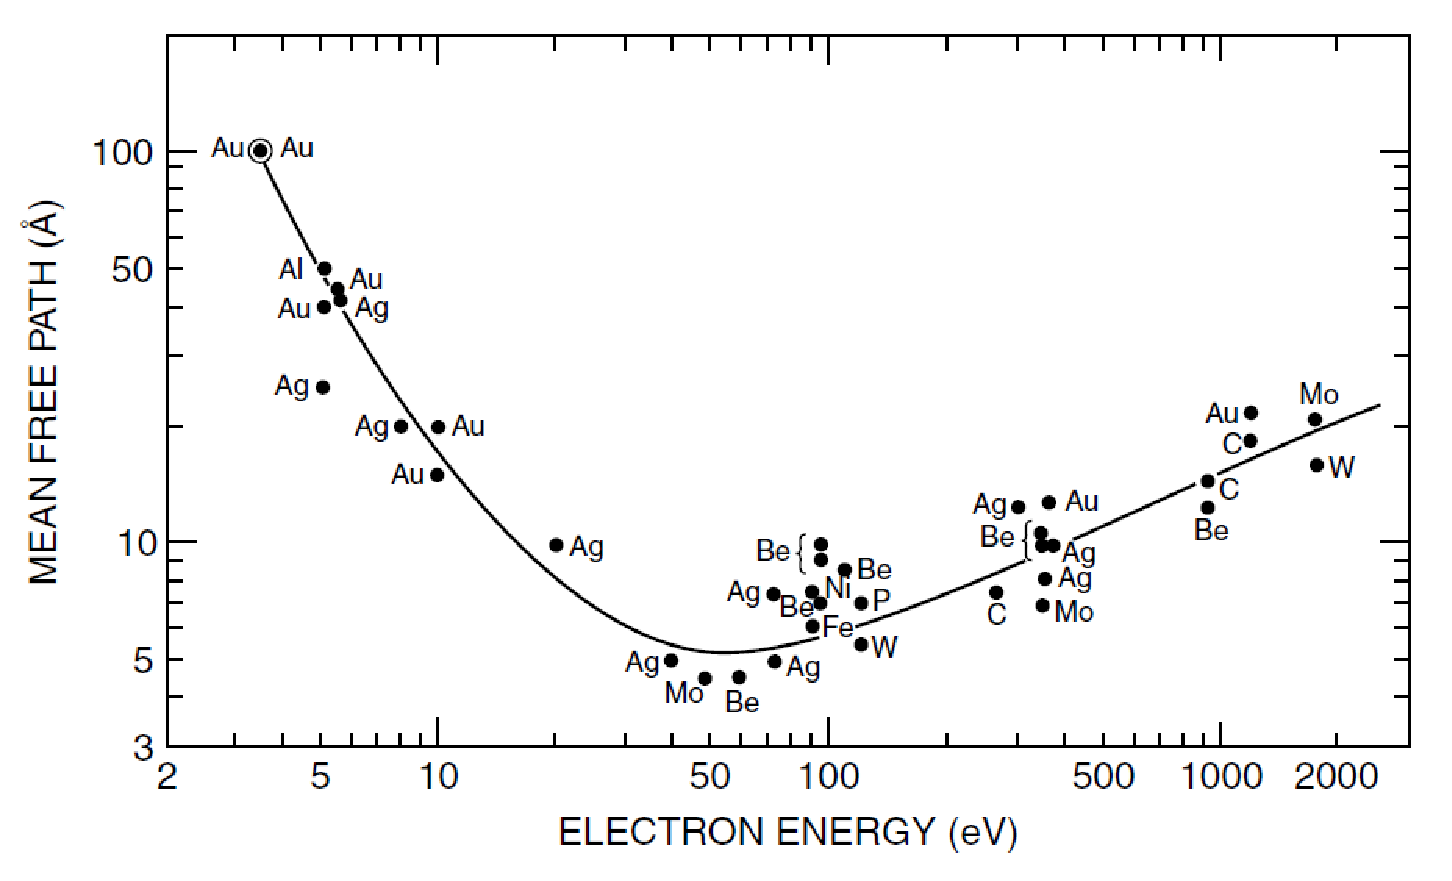
\includegraphics[scale=0.4]{img/ucurve}
\caption{Universal curve of electron escape depth \label{fig:ucurve}}
\end{figure}

\subsection{The XPS spectrum}

Figure~\ref{fig:spectrum} shows a sample XPS spectrum, where (a) are peaks from emissions of core level electrons, (b) are peaks from Auger processes, (c) are peaks from emission of valence band electrons and (d) are peaks secondary electron electron excitation and inelastic scattering processed.

\begin{figure}
\centering
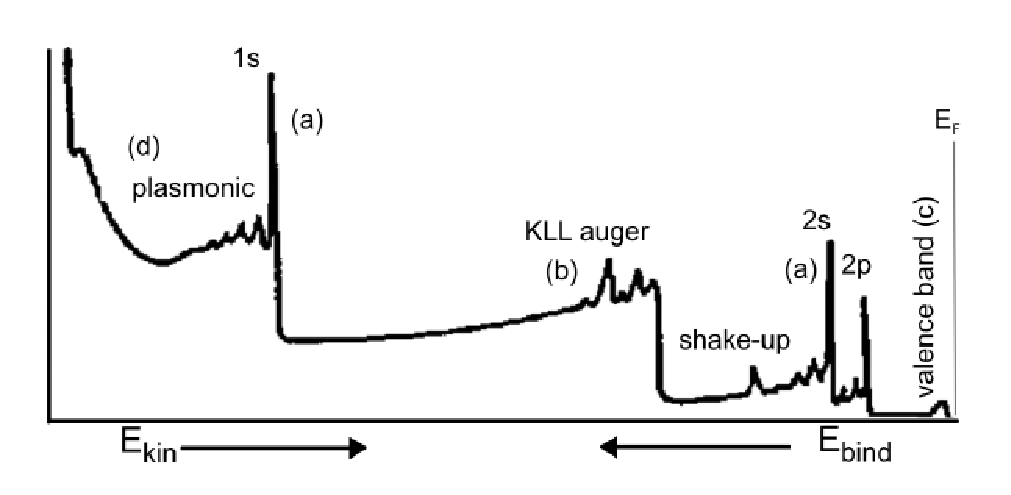
\includegraphics[scale=0.4]{img/spectrum}
\caption{Sample XPS spectrum \label{fig:spectrum}}
\end{figure}

\subsubsection{The Photoelectric Effect}

The grand structure of the XPS spectrum is supplied by the multiplett structure (as described in the following section) that is probed by the simple photoelectric effect.

In the photoelectric effect a single electron absorbs a single photon and is excited in the vacuum with the kinetic energy:
\begin{equation}
E_{kin} = \hbar \nu - E_{B} - \Phi,
\end{equation}
where the first term on the right-hand side gives the energy of the incoming photon, the second term $E_{B}$ gives the binding energy of the electron measured with respect to the Fermi energy and the last term $\Phi$ gives the work function of the material, which is the difference between the Fermi and vacuum level, i.e. the minimum energy to excite an electron from the material.

The binding energy of a material is different to the one of a free atom of this element. It is given by
\begin{equation}
E_{B} = E_{B,atom} + \Delta E_{chem} + \Delta E_{lattice} + \Delta E_{ref}, \label{eq:binding}
\end{equation}
where $\Delta E_{chem}$ gives the chemical shift, due to neighboring atoms, $\Delta E_{lattice}$ gives the difference due electrostatic interactions in the lattice (usually called the Madelung constant) and $\Delta E_{rel}$ subsumes many-body effects in the final 1-hole state.

\subsection{Spin-Orbit Coupling}

To fully describe an electron's energy in an atom---and by that the multiplett structure of the XPS spectrum---one has to account for magnetic moments of the electron. Each electron has a magnetic moment due to its orbital movement in the atom and another one due to its spin. All of these magnetic moments of all electrons interact and lead to energy shifts in the spectra. For light atoms the spin-orbit interaction can be approximated by an interaction of the total angular momentum and the total spin (L-S-coupling), which is possible when the coupling of individual spins and orbital angular momenta is negligible. The part of the Hamiltonian describing spin-orbit coupling is then given by
\begin{equation}
H_{SL} = - \frac{\mu_B}{\hbar m_e e c^2}\frac{1}{r}\frac{\partial V(r)}{\partial r} \boldsymbol{L}\cdot\boldsymbol{S},
\end{equation}
where $\mu_B$ is the Bohr magneton, $m_e$ is the electron mass, $e$ is the elementary charge, $c$ is the speed of light, $V$ is the core potential and $r$ is the distance of the electron to the nucleus.
For heavier atoms the coupling between individual spin and orbital momenta is non-negligible and a better approximation is the coupling of individual total angular moment $J_i=L_i+S_i$, this is called J-J-coupling. 

As our samples will be made of heavier elements, J-J-Coupling is the better approximation. Thus all emission lines of full electron shells in the ground state will split in doublets for $(l+\tfrac{1}{2})$ and $(l-\tfrac{1}{2})$. In principle for s-shells with $l=0$ no splitting would occur, but an effect called magnetic spin-spin exchange splitting, leads to a doublet splitting of s-shells through the interaction partially filled shells.


\subsubsection{Inner-Shell Excitations and the Auger Effect}

If a core electron is excited, one possible relaxation process is the emission of an Auger electron. In this relaxation process an electron from a higher shell fills the core hole and the emitted photon is absorbed by another electron in a higher shell that is thus excited in the continuum. The resulting atom is doubly ionized. 

The energy of the emitted Auger electron is given by
\begin{equation}
E_{kin} = E(K)-E(L)-E'(L') = E(K)-E(L)-E(L')-C(LL',T)+R
\end{equation}
where the $E(K)$ is the binding energy of the core electron, $E(L)$ is the binding energy of the electron filling the core hole. $E'(L')$ is the effective binding energy of the electron that is emitted as Auger electron. The effective binding energy consists of the binding energy of the shell $E(L')$, a coupling energy between the holes at $L$ and $L'$ and the final state $T$ and a so-called electronic relaxation $R$. It is important to note that the kinetic energy of the Auger electron is only dependent on the participating states of the Auger process and not on the energy of the particle that initially excites the core electron.

\subsubsection{Plasmons}

A plasmon is a quasi-particle coming up in condensed matter, describing quantized plasma oscillations, i.e. oscillations of the electron gas as a whole. The excitation energy of plasmons is specific to all materials and are given by the materials plasma frequency, both of which are tabulated and can be looked up. 

For a free electron gas the bulk plasma frequency is given by
\begin{equation}
\omega_{b} = \sqrt{\frac{e^2 n}{m_e \epsilon_0}},
\end{equation}
where $e$ is the elementary charge, $\epsilon_0$ the permittivity of free space, $m_e$ the mass of the electron and $n$ the conduction electron density. Apart from the 3-dimensional case also surface plasmons, excitations of the electron gas restricted to the surface, can be excited.

An electron having excited one or more plasmons is said to have suffered plasmon loss. This is one reason for satellites to ``real'' peaks in spectra.

\section{Experimental Setup}

In this section we will describe shortly the machinery and techniques used in this experiment. A schematic of the setup is shown in figure~\ref{fig:setup}.

\begin{figure}
\centering
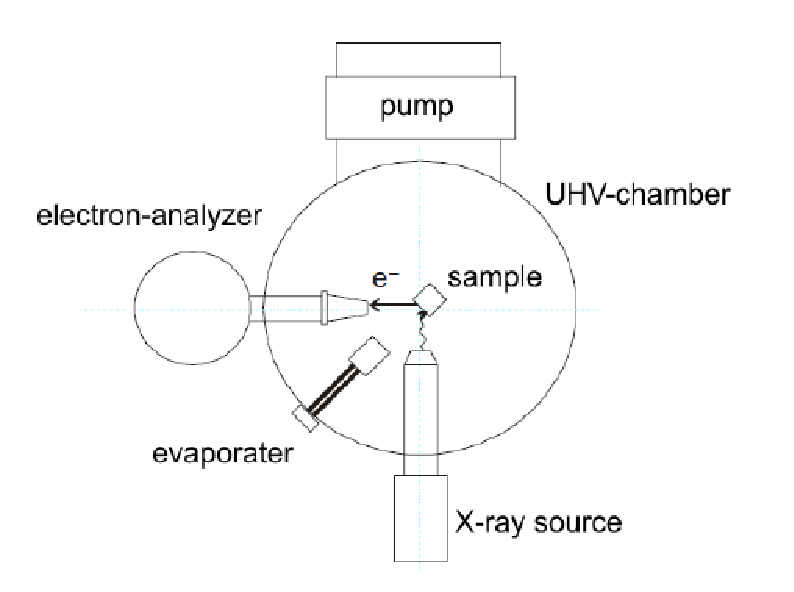
\includegraphics[scale=0.4]{img/setup}
\caption{Schematic setup of the experiment \label{fig:setup}}
\end{figure}


\subsection{Ultra High Vacuum (UHV)}

This experiment needs an ultra high vacuum environment for two reasons. First, electrons have very short mean free path in matter, as can be seen in figure~\ref{fig:ucurve}. Second, the higher the pressure the faster gas atoms from the rest atmosphere in the chamber adsorb to the sample, this is again unwanted, as XPS is a very surface sensitive technique and assertions about bulk properties of samples can, if ever, only be made from properties of atomically clean surfaces.

The ultra high vacuum is usually obtained by the use of membrane, turbo molecular, ion getter pump and sublimation pumps, as well as baking of the chamber. This experiment diaphragm pump to achieve a prevacuum of about $\sim 10^{-6}\,$mbar and based on that, a turbomolecular pump to achieve a vacuum of about $10^{-9}\,$mbar. The final pressure of about $10^{-10}\,$mbar is achieved through baking.

\paragraph{The Diaphragm Pump} is a rather simple mechanical pump. A membrane is moved up and down in conjunction with two valves opening and closing openings to the chamber and the environment, thus sucking gas from the chamber into the pump and pushing it out to the environment.

\paragraph{The Turbomolecular Pump} is another type of mechanical pump. It consists of several stages of rotors and stators. The rotors are tilted blades rotating at a velocity approximately equal to that of the gas particles and the stators are stationary blades tilted in the other direction orthogonal to the rotors. The working principle of this pump is to transfer momentum to the gas particles in a way such that the particles are ``kicked'' out of the chamber; the tilt of the rotors is such that the momentum of the kicked particles points outward the chamber.

\paragraph{Baking} is the technique through which the final pressure is achieved. The remaining pressure achieved through the use of pumps is mainly due to water molecules still in the chamber. Due to their polarity, these water molecules are usually located at the chamber walls. By cycles of heating and cooling of the chamber they can be pumped out. This procedure can take several days, which makes it of utmost importance to maintain the UHV after it is obtained.

\subsection{X-Ray Source}

The X-ray source used in this experiment is made of a filament from which electrons are emitted by thermal excitation. These electrons are then accelerated and hit an anode, either aluminum or magnesium, were they produce characteristic X-ray radiation by excitation of core level electrons in the anode and a continuous X-ray spectrum through Bremsstrahlung.

The continuous X-ray radiation is filtered out by usage of an Aluminum window, about $1\,\mu$m thick, and only the characteristic spectrum is used of spectroscopy~\cite{skript}. The energy of X-rays from the aluminum anode is $1486.6\,$eV with a linewidth of $0.86\,$eV and the energy of X-rays from the magnesium anode is $1253.6\,$eV with a linewidth of $0.7\,$eV.

\subsection{Electron Energy Analyzer}

This experiment uses a hemispherical electron analyzer, as shown in figure~\ref{fig:analyzer}. The analyzer consists of two hemispherical capacitors between which an electric field is applied, thus changing the trajectory of electrons coming in through the first aperture. The strength of this field is varied such that only electrons in a certain energy range pass through the second aperture.

Before entering through the first aperture a pass voltage can be applied to the electrons, which is useful because most detectors are more accurate at lower energies, therefore a constant energy offset can be used to increase the accuracy of the measurement an order of magnitude.

The final electron detector is a channeltron, which is a  continuous version of a dynode electron multiplier. The channeltron is basically a thin glass cone coated with a semiconducting material. The signal is amplified by emission of secondary electrons, which multiplies the number of electrons in the channeltron that finally arrive at the anode. The electron multiplication is usually of the order $10^6$ to $10^9$~\cite{book}.

\begin{figure}
\centering
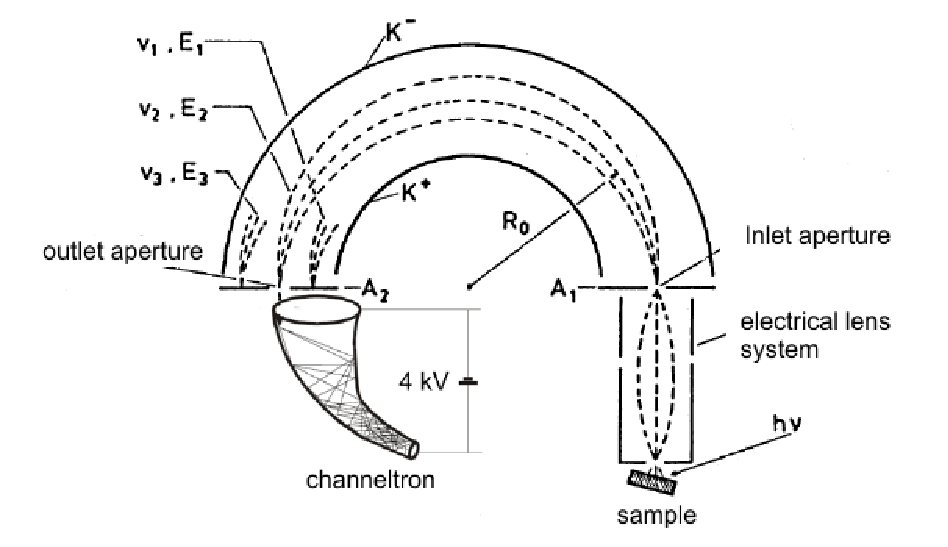
\includegraphics[scale=0.4]{img/analyzer}
\caption{Schematic of a hemispheric electron analyzer \label{fig:analyzer}}
\end{figure}

\section{Data Analysis}

In this section we will discuss we will analyze the results obtained in the experiment. For pedagogical reasons we will start with the discussion of the samarium sample, go on to the silver sample and lastly discuss the 10-DM memorial coin.

The Fermi level is obtained from all spectra by the same method described shortly in the beginning of the following section. 

All plots of spectra will be marked both with the kinetic and the binding energy. The peak positions were obtained from the spectra by zooming in on parts of the spectrum and guessing the first moment of the peak. This was feasible, because peaks are usually a few bins wide and the error in visual inspection with linear interpolation between points in the spectra is about half a bin width an much smaller than the error made when obtaining the Fermi level. The error, in the sense of the $\sigma$ interval for the first moment of a peak was also guessed. All tabulated peak values include this error and the error of the Fermi edge to which they are referenced, combined by Gaussian error propagation. The error of the Fermi edge is $1\,$eV for all cases. The additional error introduced by referencing to the Fermi edge will be mitigated by giving all values with an additional significant digit. All reference values, with one exception mentioned below, are taken from~\cite{handbook}. In tables we will omit the  explicit name of the Auger process, when listing one, since they usually cluster at certain energies  so we compare the peak of lowest binding energy, that is identified as an Auger peak by comparison to another spectrum, to the Auger peak of lowest binding energy in~\cite{handbook}.

\subsection{Samarium}

This sample consisted of a steel plate on which a fresh film of samarium was evaporated.

\subsection*{Samarium Fermi Edge}

The relevant samarium spectra are shown in figures~\ref{fig:sm_fermi}, \ref{fig:sm_al} and \ref{fig:sm_mg}. Figure~\ref{fig:sm_fermi} shows a spectrum of the samarium Fermi edge taken in an energy interval from $1450\,$eV to $1499.53\,$eV at a pass voltage of $25\,$V, 30 runs, 100 measurement points in the energy interval and a dwell time of $500\,$ms per point. This low pass voltage was set to obtain a high resolution, but this also warranted the need to sum the large number of spectra and the large dwell time, so as to decrease the influence of statistical fluctuations.

We will also use this spectrum to  explain how we obtained the Fermi edge. We search for the most outward peak or a significant step at a high kinetic energies in the spectrum, somewhere in the range of $5$--$10\,$eV below the energy of the incident X-rays. We then looked at the maximal peak intensity and the average base intensity at higher kinetic energies after that. We then used the energy at half the difference in intensity as the Fermi edge and guesses an error for this position, so that more than two thirds of the intensity difference where were achieved from either direction. This amounts to the thick line in figure~\ref{fig:sm_fermi} at $1476.5\,$eV and the two dashed lines at $1476.5 \pm 1\,$eV.

The Fermi edge at $1476.5\,$eV is  $10.2\,$eV lower than the energy of the incident photons, but \textit{Wolfram Alpha} gives the work function of Samarium  as $2.7\,$eV which gives a difference of $(7.5 \pm 1.0)\,$eV. This difference is not specific to this sample or the aluminum anode, but shifts of the Fermi edge of about this order of magnitude will be observed for all sample-anode-material combinations. This hints to several possible error sources, like an electrical charging of the samples, chemical shifts and systematic errors in the electron energy analyzer. We will discuss this point further in the conclusion.

We also fitted two overlapping Lorentzians (according to~\cite{book}) with the Levenberg-Marquardt algorithm to obtain the position of the $4f$ and $5p$ energy levels. The obtained binding energies and their errors from the fits including the error of the Fermi level are $(3.2 \pm 1.0)\,$eV for the $4f$ state and $(19.6 \pm 1.0)\,$eV for the $5p$ state. \cite{handbook} gives the energy of the $5p$ state as $19\,$eV, which is compatible, but no data for the $4f$ state are given. A  binding energy of $5.2\,$eV for the $4f$ state an $21.2\,$eV for the $5p$ state were found in~\cite{booklet}, both of which are incompatible with our measurements, as our values are smaller. The point of systematically smaller values in our measurements will repeat throughout this experiment.

\begin{figure}
\centering
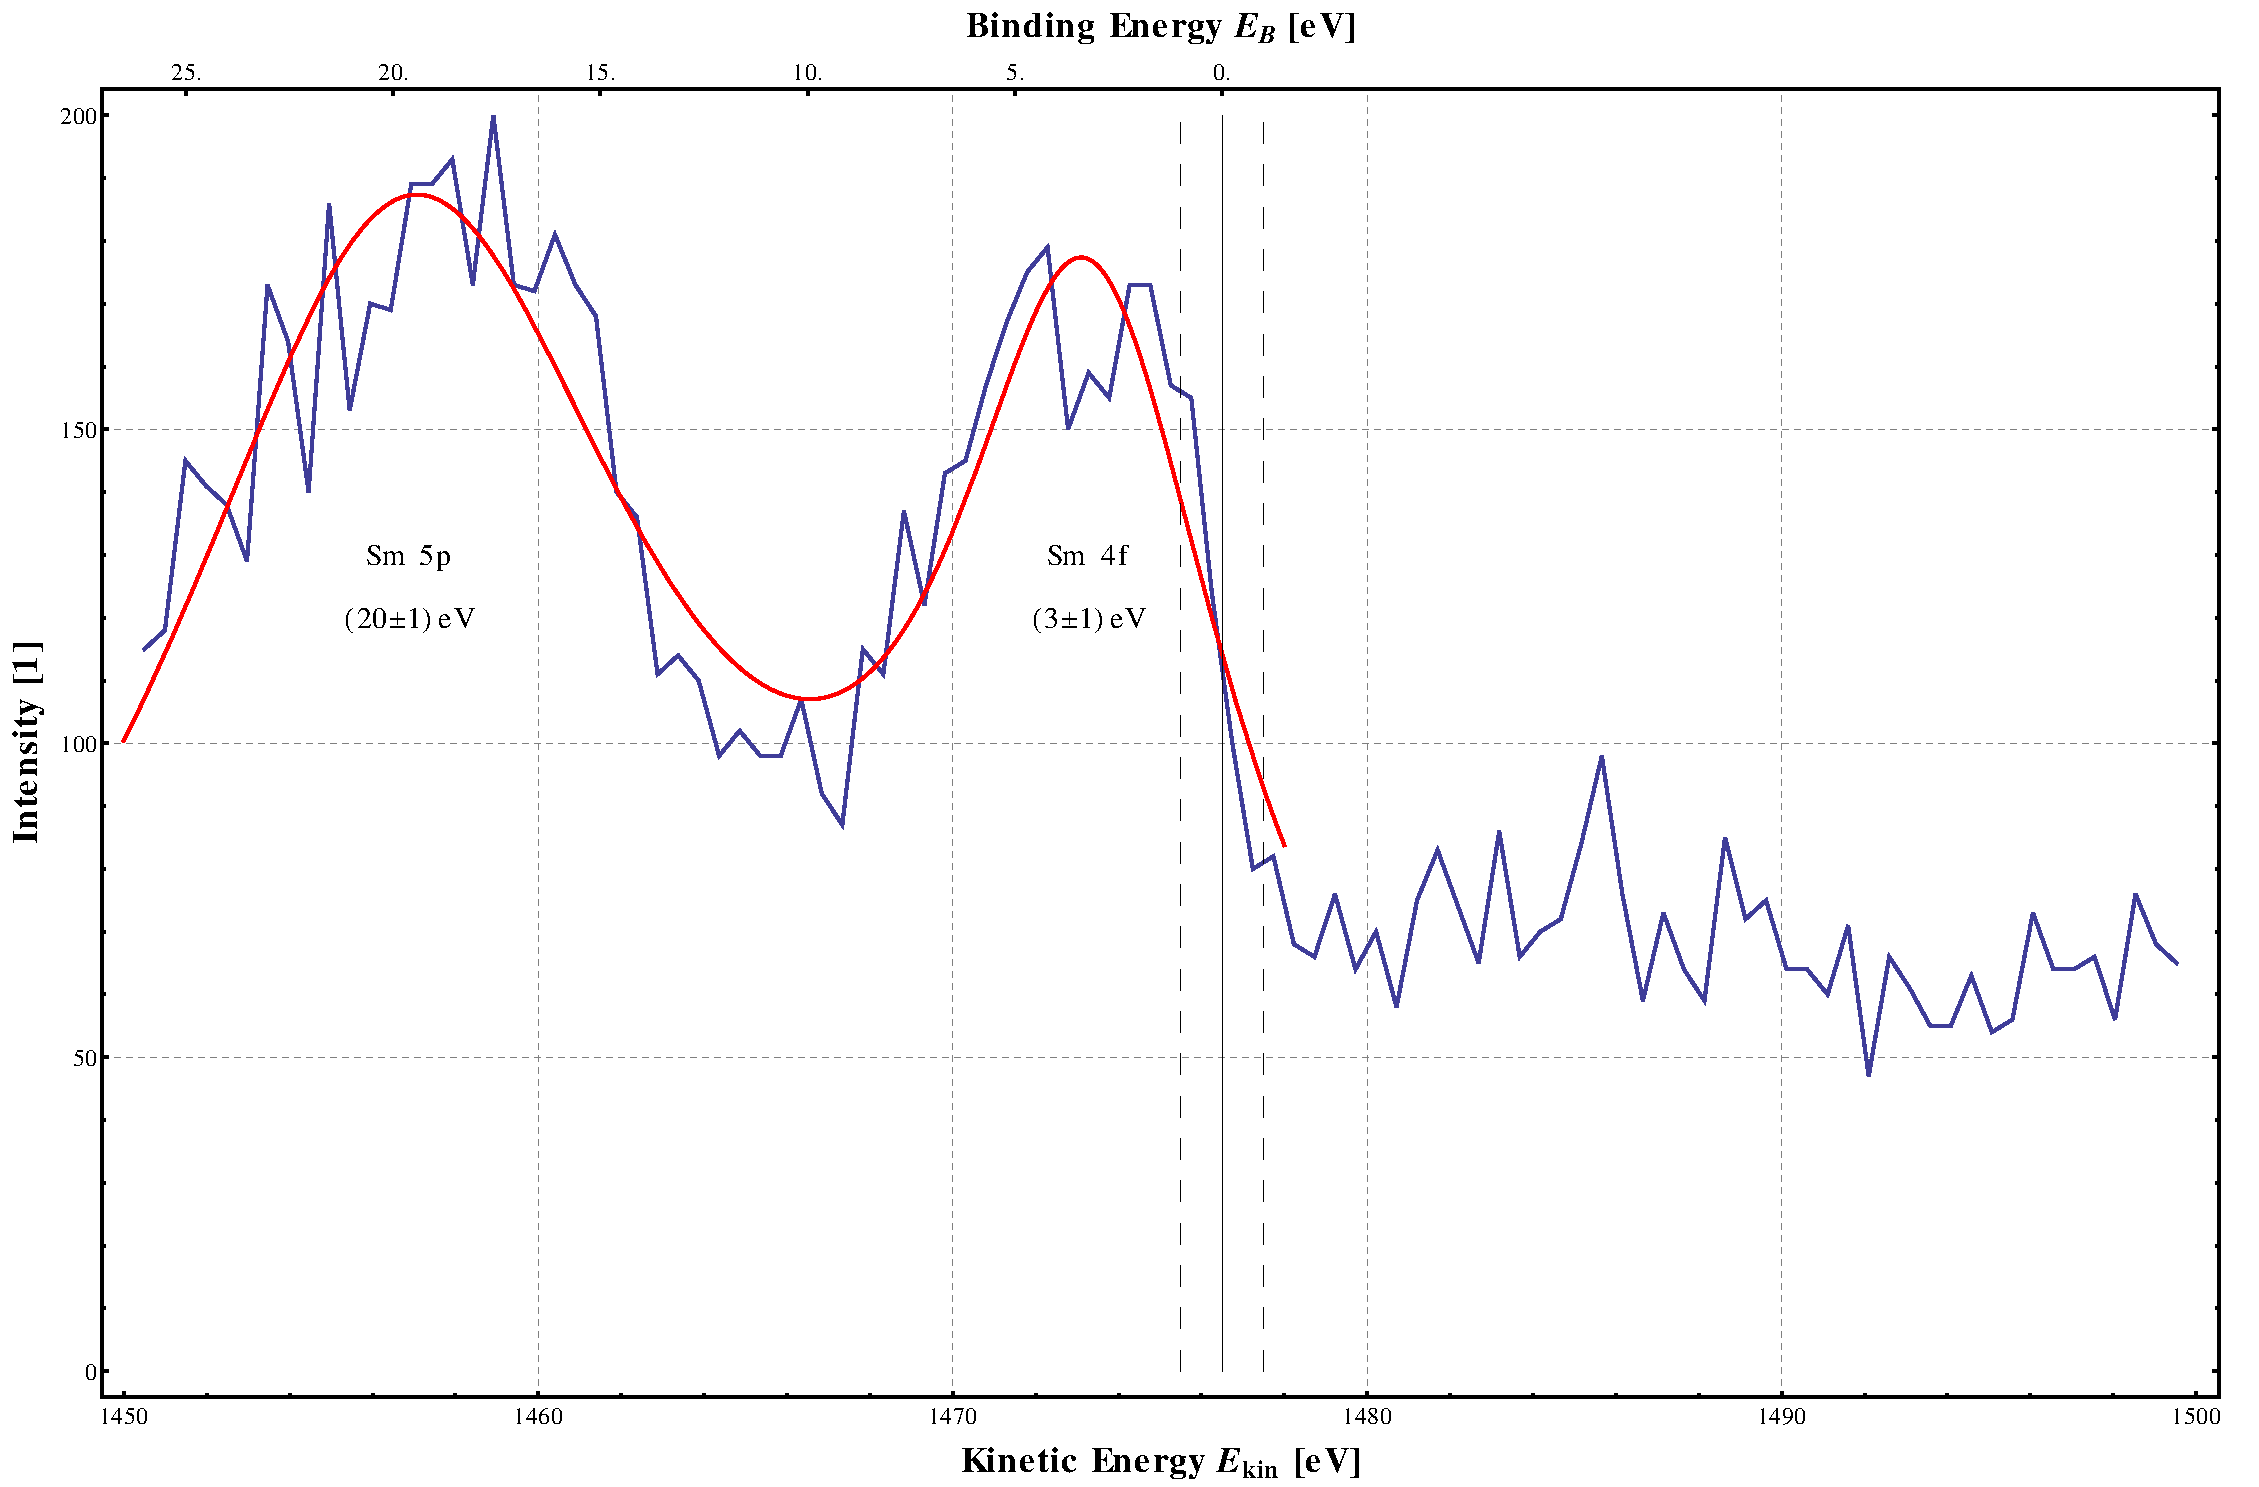
\includegraphics[scale=0.3]{img/samarium_fermiedge_al}
\caption{Spectrum of the samarium Fermi edge and 4f and 5p state \label{fig:sm_fermi}}
\end{figure}

\subsection*{Samarium Al-K$_{\alpha}$ Spectrum}

Figure~\ref{fig:sm_al} shows an overview Al-K$_{\alpha}$ spectrum of samarium taken in the energy range of $200$--$1488.5\,$eV at a pass voltage of $50\,$V with 7 runs, a dwell time per point of $333\,$ms and 1300 points in the energy interval. 

All peaks, that could be identified are found in table~\ref{tab:sm_al_ident}. For the identification of the photopeaks we used~\cite{handbook}; the Auger peaks were identified in conjunction with the Mg-K$_{\alpha}$ spectrum discussed in the next section, because Auger peaks lie at the same kinetic energies in spectra taken at different energies of incident X-rays, since they are emitted at discrete, very precise, element specific energies. 

The only element we can identify on top of samarium is oxygen which points to a slight oxidization of the sample. Iron, the main ingredient of steel, could not be found, which is not surprising since XPS is a surface sensitive technique and later spectra will hint, that enough samarium has been deposited in the chamber by now. All peak positions are systematically shifted to lower binding energies, but not by a constant offset, but a certain percentage between one and two percent.

\begin{figure}[h]
\centering
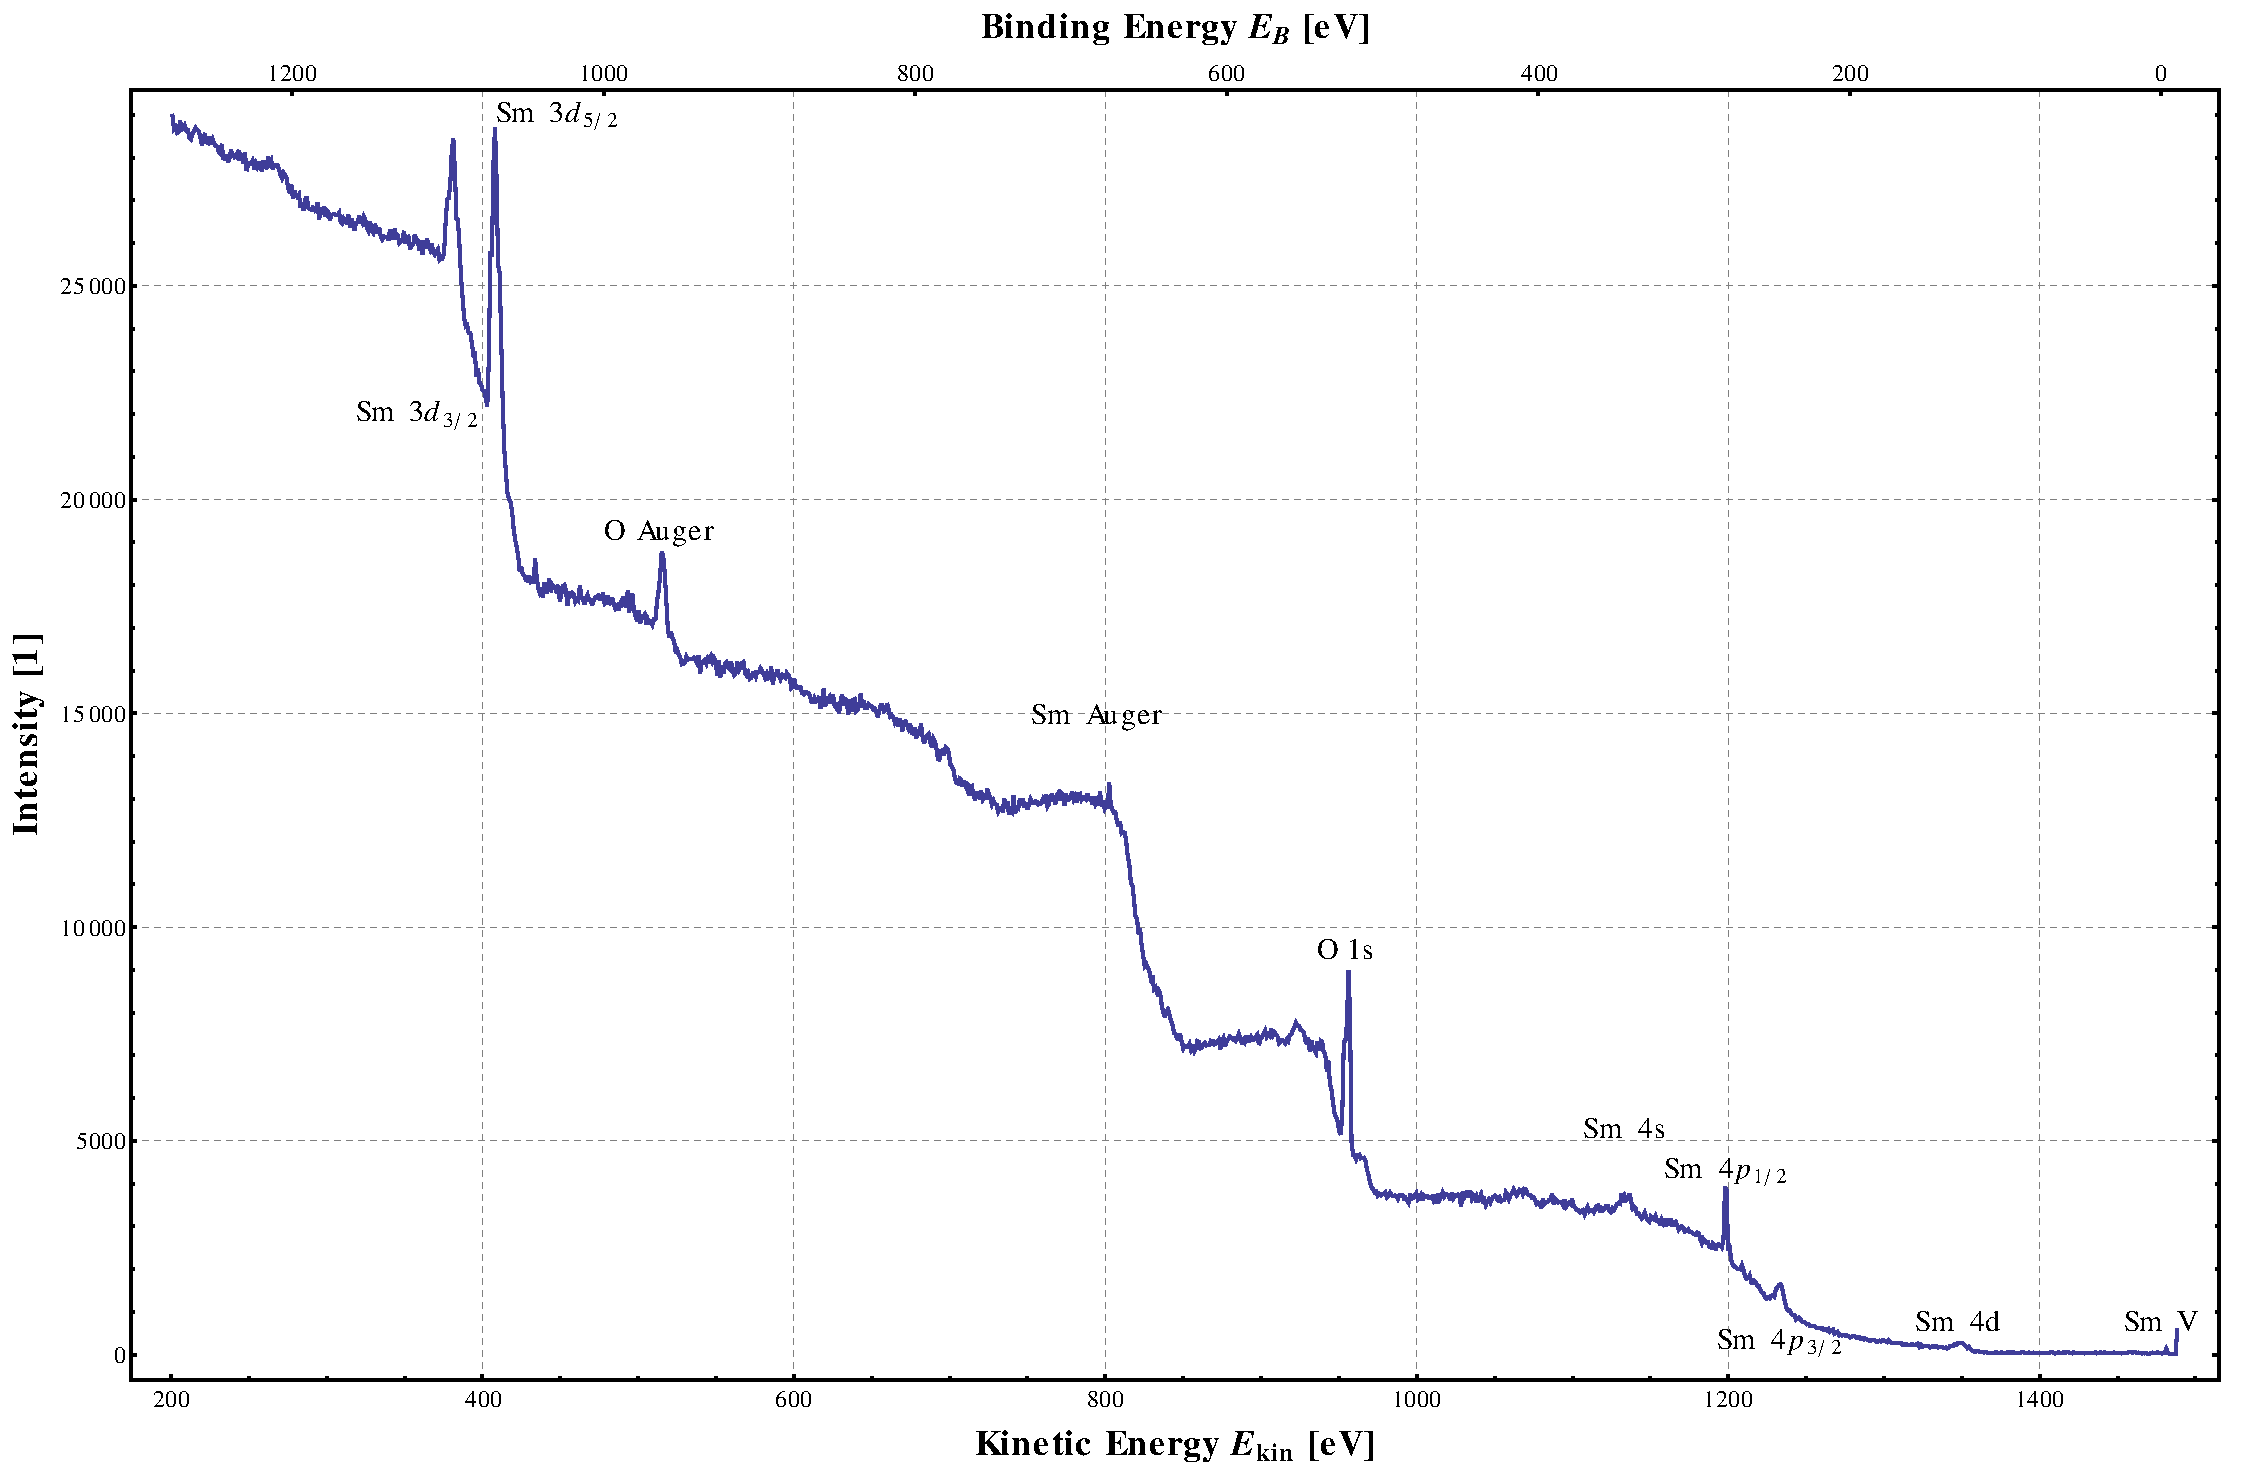
\includegraphics[scale=0.3]{img/samarium_binding_al}
\caption{Spectrum of samarium sample taken with aluminum anode \label{fig:sm_al}}
\end{figure}

\begin{table}[h]
\begin{center}
\begin{tabular}{lcccc}
\toprule
Measured $E_{B}$ [eV]      & Identification & Theoretical$E_{B}$ [eV] & Abs. Dev. [eV] & Dev. [\%]\\
\midrule
\phantom{0}128.0 $\pm$ 1.5 & Sm $4d$        & 129                     & $-1.0$         & $-0.8$\\
\phantom{0}243.5 $\pm$ 2.3 & Sm $4p_{3/2}$  & 250                     & $-6.5$         & $-2.6$\\
\phantom{0}278.0 $\pm$ 1.5 & Sm $4p_{1/2}$  & 283                     & $-5.0$         & $-1.8$\\
\phantom{0}343.0 $\pm$ 2.3 & Sm $4s$        & 349                     & $-6.0$         & $-1.7$\\
\phantom{0}521.5 $\pm$ 1.9 & O $1s$         & 531                     & $-9.5$         & $-1.8$\\
\phantom{0}677.5 $\pm$ 5.1 & Sm Auger       & 682                     & $-4.5$         & $-0.7$\\
\phantom{0}961.0 $\pm$ 1.5 & O Auger        & 978                     & $-17.0$        & $-1.7$\\
1068.5 $\pm$ 1.9           & Sm $3d_{5/2}$  & 1081                    & $-12.5$        & $-1.2$\\
1095.5 $\pm$ 1.9           & Sm $3d_{3/2}$  & 1108                    & $-12.5$        & $-1.1$\\
\bottomrule
\end{tabular}
\end{center}
\par
\caption{Binding energies obtained from samarium spectrum taken with aluminum anode from figure~\ref{fig:sm_al} \label{tab:sm_al_ident}}
\end{table}


\subsection*{Samarium Mg-K$_{\alpha}$ Spectrum}

Figure~\ref{fig:sm_mg} shows an overview Mg-K$_{\alpha}$ spectrum of samarium taken in the energy range of $199.85$--$1289.84\,$eV at a pass voltage of $50\,$V with 2 runs, a dwell time per point of $333\,$ms and 1100 points in the energy interval. 

The Fermi energy was found at $(1247.5 \pm 1.0)\,$eV which is $(3.4 \pm 1.0)\,$eV. The peaks we could identify can be found in table~\ref{tab:sm_mg_ident}. Additionally to samarium and oxygen we found three peaks labeled X1, X2 and X3 for which now sensible choices for the element of origin could be found in either~\cite{handbook} or \cite{nist}. Also figure~\ref{fig:sm_mg} shows two very narrow peaks at binding energies higher than $900\,$eV that are labeled ``shady peaks''. We believe these to be the results of charged elementary particles, e.g. a cosmic muon, hitting the channeltron from the outside.

The identified peaks are shifted, as for the aluminum anode, systematically to lower values; by the same percentage.

\begin{figure}[h]
\centering
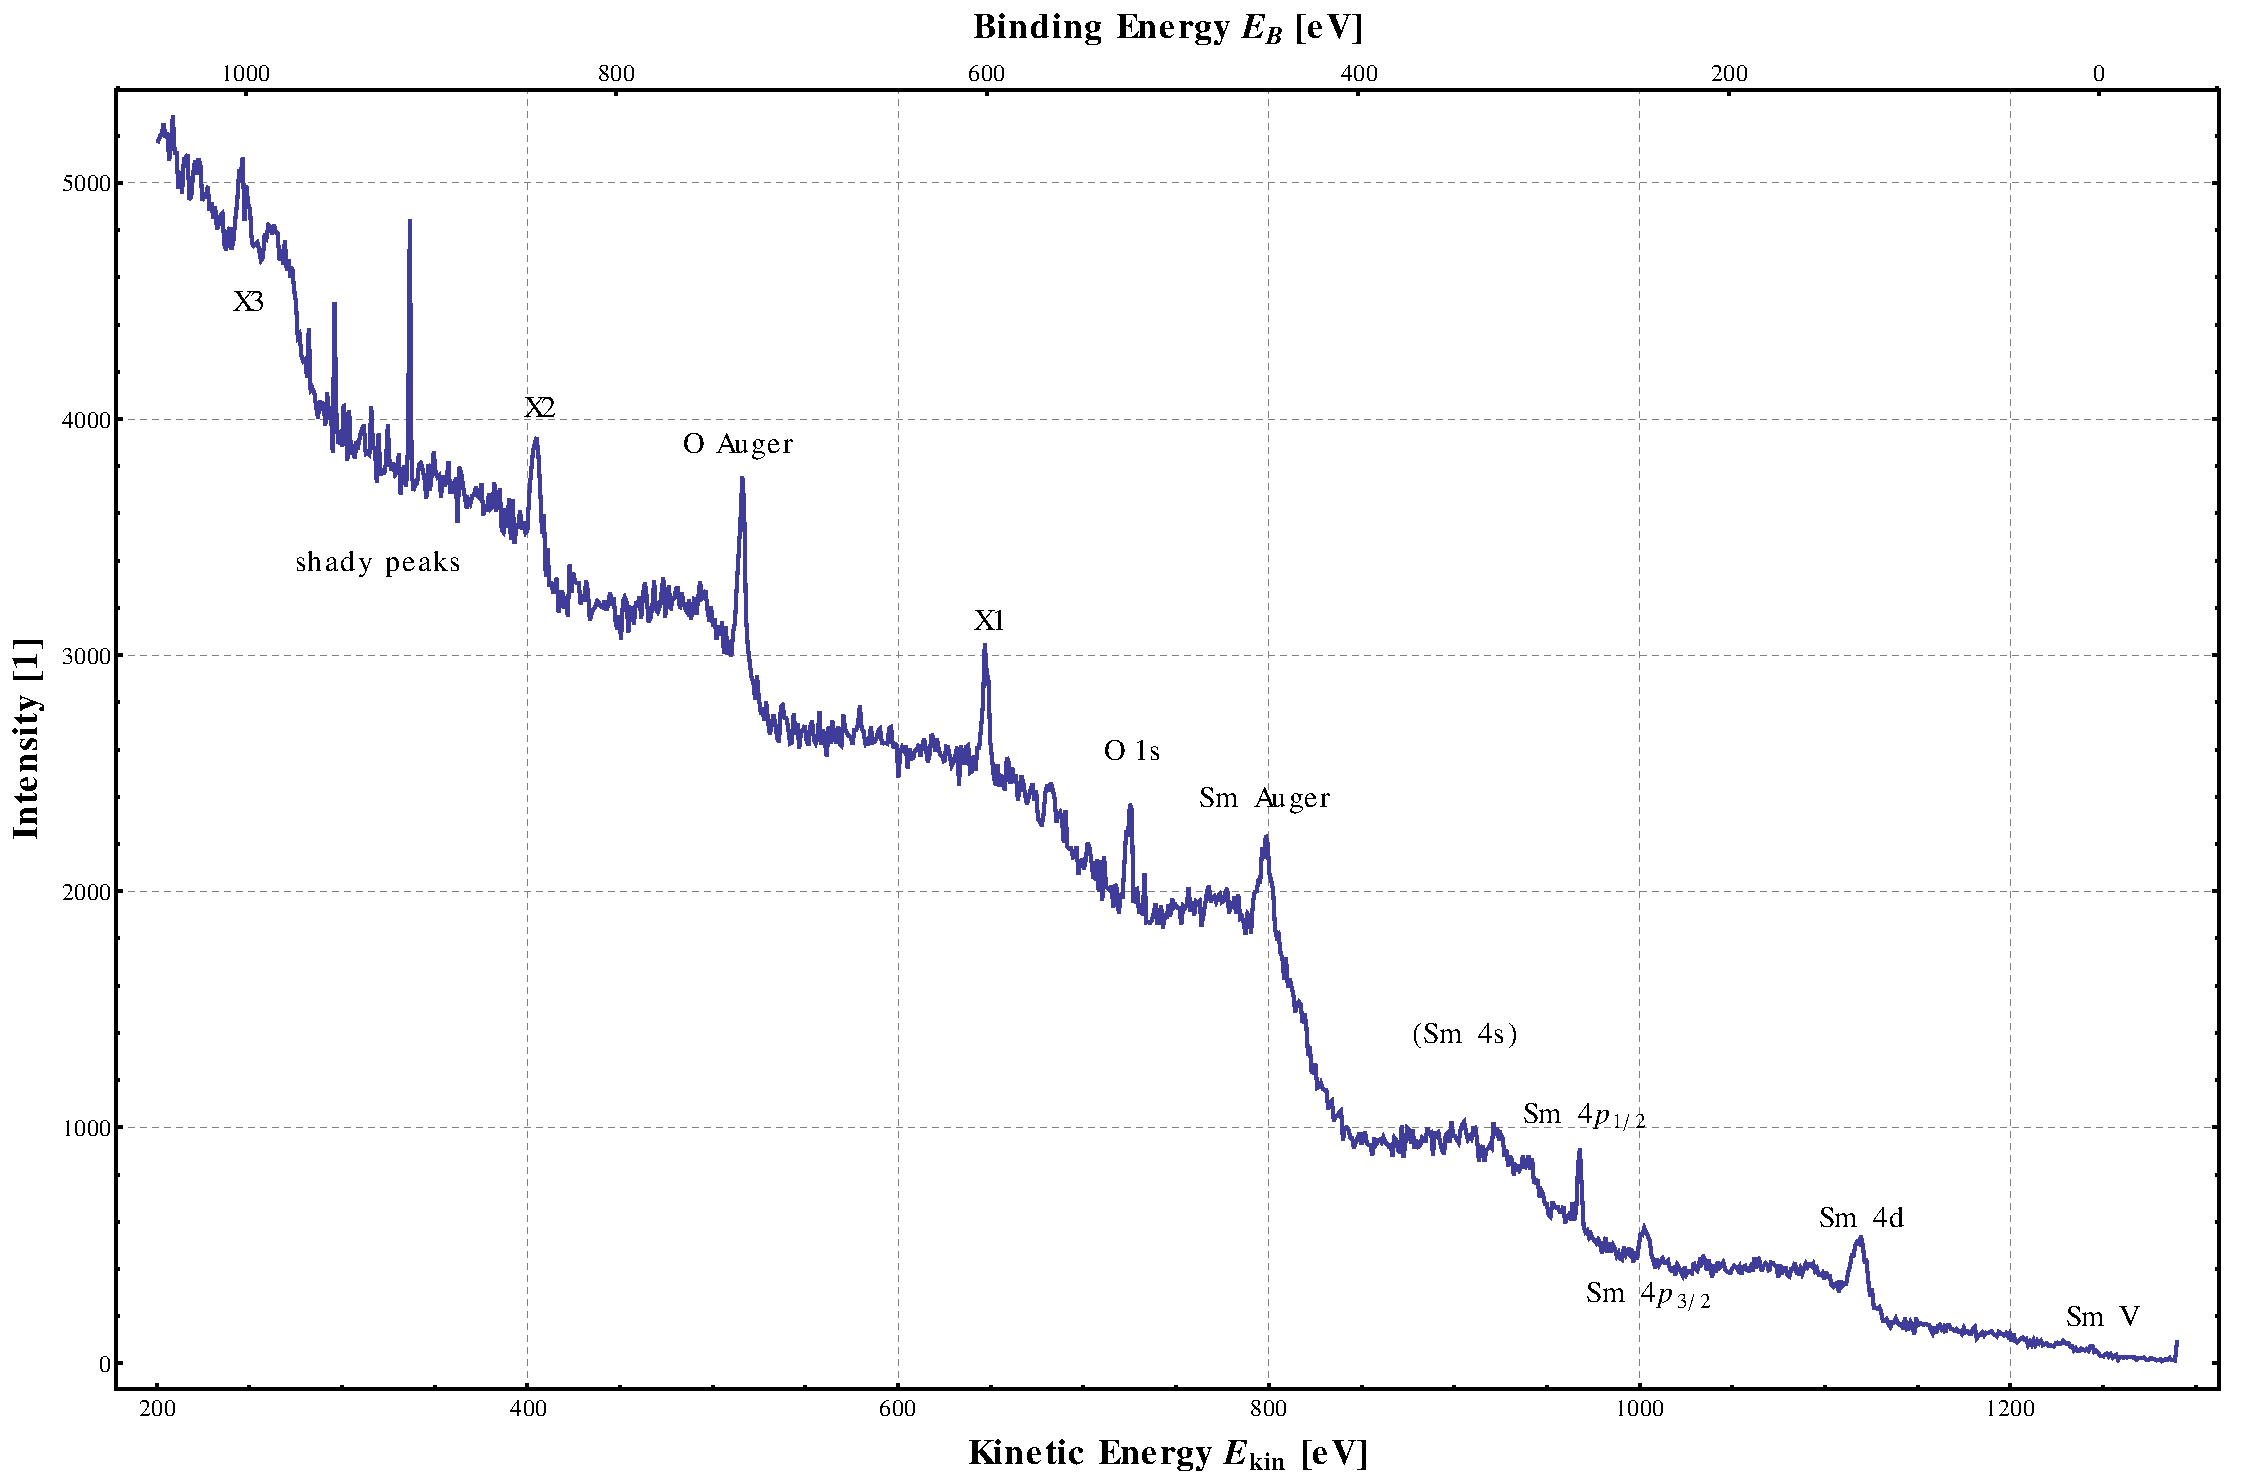
\includegraphics[scale=0.3]{img/samarium_binding_mg}
\caption{Spectrum of samarium sample taken with magnesium anode \label{fig:sm_mg}}
\end{figure}

\begin{table}[h]
\begin{center}
\begin{tabular}{lcccc}
\toprule
Measured $E_{B}$ [eV]      & Identification & Theoretical$E_{B}$ [eV] & Abs. Dev. [eV] & Dev. [\%]\\
\midrule
\phantom{0}129.0 $\pm$ 2.3 & Sm $4d$        & 129                     & $0.0$          & $0.0$ \\
\phantom{0}245.0 $\pm$ 1.9 & Sm $4p_{3/2}$  & 250                     & $-5.0$         & $-2.0$\\
\phantom{0}280.0 $\pm$ 1.5 & Sm $4p_{1/2}$  & 283                     & $-3.0$         & $-1.1$\\
\phantom{0}342.0 $\pm$ 5.1 & Sm $4s$        & 349                     & $-7.0$         & $-2.0$\\
\phantom{0}449.5 $\pm$ 2.3 & Sm Auger       & 449                     & $0.5$          & $0.1$ \\
\phantom{0}523.0 $\pm$ 1.9 & O $1s$         & 531                     & $-8.0$         & $-1.5$\\
\phantom{0}600.0 $\pm$ 1.5 & X1             &                         &                &       \\
\phantom{0}731.5 $\pm$ 1.9 & O Auger        & 745                     & $-13.5$        & $-1.8$\\
\phantom{0}843.0 $\pm$ 2.3 & X2             &                         &                &       \\
1000.0 $\pm$ 1.5           & X3             &                         &                &       \\
\bottomrule
\end{tabular}
\end{center}
\par
\caption{Binding energies obtained from samarium spectrum taken with magnesium anode from figure~\ref{fig:sm_mg} \label{tab:sm_mg_ident}}
\end{table}


\subsection{Silver}

This sample is a simple piece of silver. \textit{Wolfram Alpha} gives the work function of silver as $4.52$--$4.74\,$eV, for simplicity we will use a value of $4.6\,$eV.

\subsection*{Silver Al-K$_{\alpha}$ Spectrum}

Figure~\ref{fig:ag_mg} shows an overview Al-K$_{\alpha}$ spectrum of silver taken in the energy range of $200$--$1488.5\,$eV at a pass voltage of $50\,$V with 2 runs, a dwell time per point of $333\,$ms and 1100 points in the energy interval. 

The Fermi edge  was found at a kinetic energy of $(1478.0 \pm 1.0)\,$eV, which gives gives difference of $6\,$eV to the energy of the incident photons minus the work function.

The identified peaks can be found in table~\ref{tab:ag_al_ident}. In addition to the photo- and Auger peaks of silver we can also find  peaks corresponding to oxygen and samarium, which is sensible since samarium has been evaporated into the chamber for a long time very regularly. The samarium $4p_{1/2}$ could also possibly be a carbon $1s$ peak, since these are ubiquitous in XPS, since organic residues can remain on samples when they are handled.

As for the previous samples we observe a systematic shift of all binding energies by about $-(1$--$2)\,\%$

\begin{figure}[h]
\centering
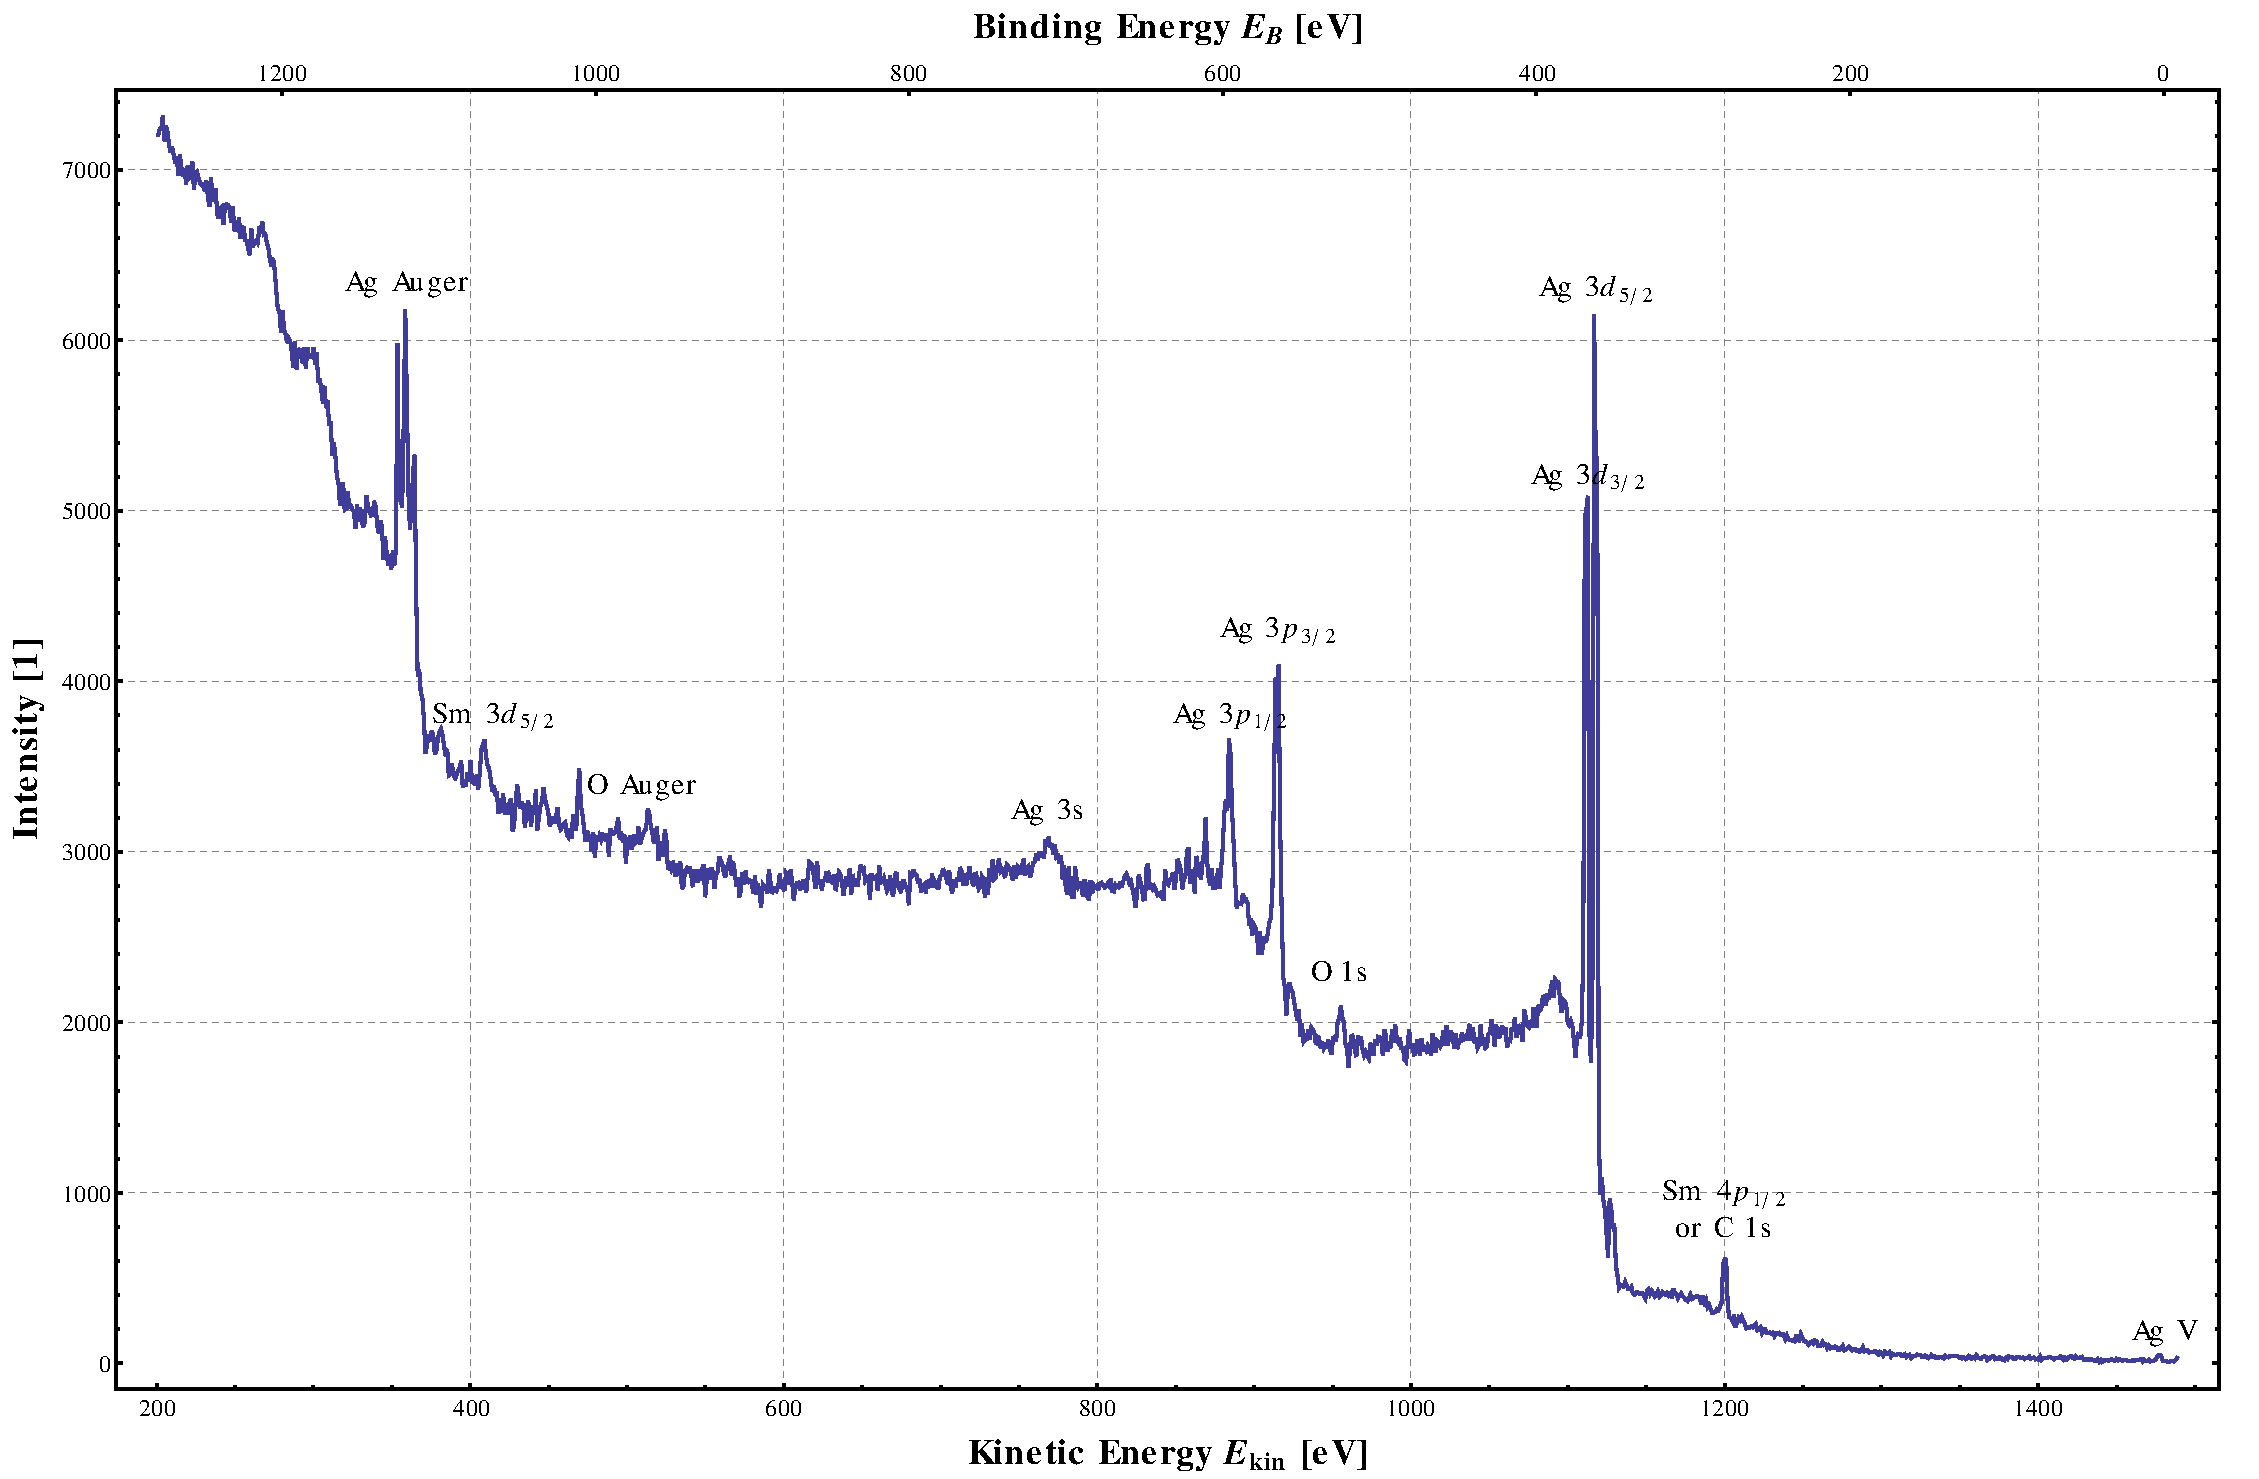
\includegraphics[scale=0.3]{img/silver_binding_al}
\caption{Spectrum of silver sample taken with aluminum anode \label{fig:ag_al}}
\end{figure}

\begin{table}[h]
\begin{center}
\begin{tabular}{lcccc}
\toprule
Measured $E_{B}$ [eV]        & Identification & Theoretical$E_{B}$ [eV] & Abs. Dev. [eV] & Dev. [\%]\\
\midrule
\phantom{0}278.0 $\pm$ 1.5   & Sm $4p_{1/2}$  & 283                     & $-5.0$         & $-1.8$\\
\phantom{0}278.0 $\pm$ 1.5   & C $1s$         & 285                     & $-7.0$         & $-2.5$\\
\phantom{0}360.5 $\pm$ 1.5   & Ag $3d_{5/2}$  & 368                     & $-7.5$         & $-2.0$\\
\phantom{0}366.0 $\pm$ 1.5   & Ag $3d_{3/2}$  & 374                     & $-8.0$         & $-2.1$\\
\phantom{0}523.0 $\pm$ 2.3   & O $1s$         & 531                     & $-8.0$         & $-1.5$\\
\phantom{0}563.5 $\pm$ 1.5   & Ag $3p_{3/2}$  & 573                     & $-9.5$         & $-1.7$\\
\phantom{0}594.5 $\pm$ 1.9   & Ag $3p_{1/2}$  & 604                     & $-9.5$         & $-1.6$\\
\phantom{0}710.0 $\pm$ 5.1   & Ag $3s$        & 712                     & $-2.0$         & $-0.3$\\
\phantom{0}969.0 $\pm$ 5.1   & O Auger        & 978                     & $-9.0$         & $-0.9$\\
1069.0 $\pm$ 2.3             & Sm $3d_{5/2}$  & 1081                    & $-12.0$        & $-1.1$\\
1113.0 $\pm$ 1.5             & Ag Auger       & 1129                    & $-16.0$        & $-1.4$\\
\bottomrule
\end{tabular}
\end{center}
\par
\caption{Binding energies obtained from silver spectrum taken with aluminum anode from figure~\ref{fig:ag_al} \label{tab:ag_al_ident}}
\end{table}

\subsection*{Silver Mg-K$_{\alpha}$ Spectrum}

Figure~\ref{fig:ag_mg} shows an overview Mg-K$_{\alpha}$ spectrum of silver taken in the energy range of $200$--$1290\,$eV at a pass voltage of $50\,$V with 3 runs, a dwell time per point of $333\,$ms and 1100 points in the energy interval. 

We determined the Fermi to be at a kinetic energy of $(1248.0 \pm 1.0)\,$eV, which gives gives difference of $1\,$eV to the energy of the incident photons minus the work function.

The identified peaks can be found in table~\ref{tab:ag_mg_ident} and support our findings from previous section. Additionally we find a copper ghost peak, hinting at copper contaminations in the magnesium anode, and a very prominent double peak at a binding energy of about $685\,$eV, that we were unable to identify. At this point we also to mention, that peaks may not always be identified blindly, since what could be identified as samarium $4s$ peak is just a normal part of the silver spectrum, as can be found in~\cite{handbook}. We also observe the typical systematic shift.

\begin{figure}[h]
\centering
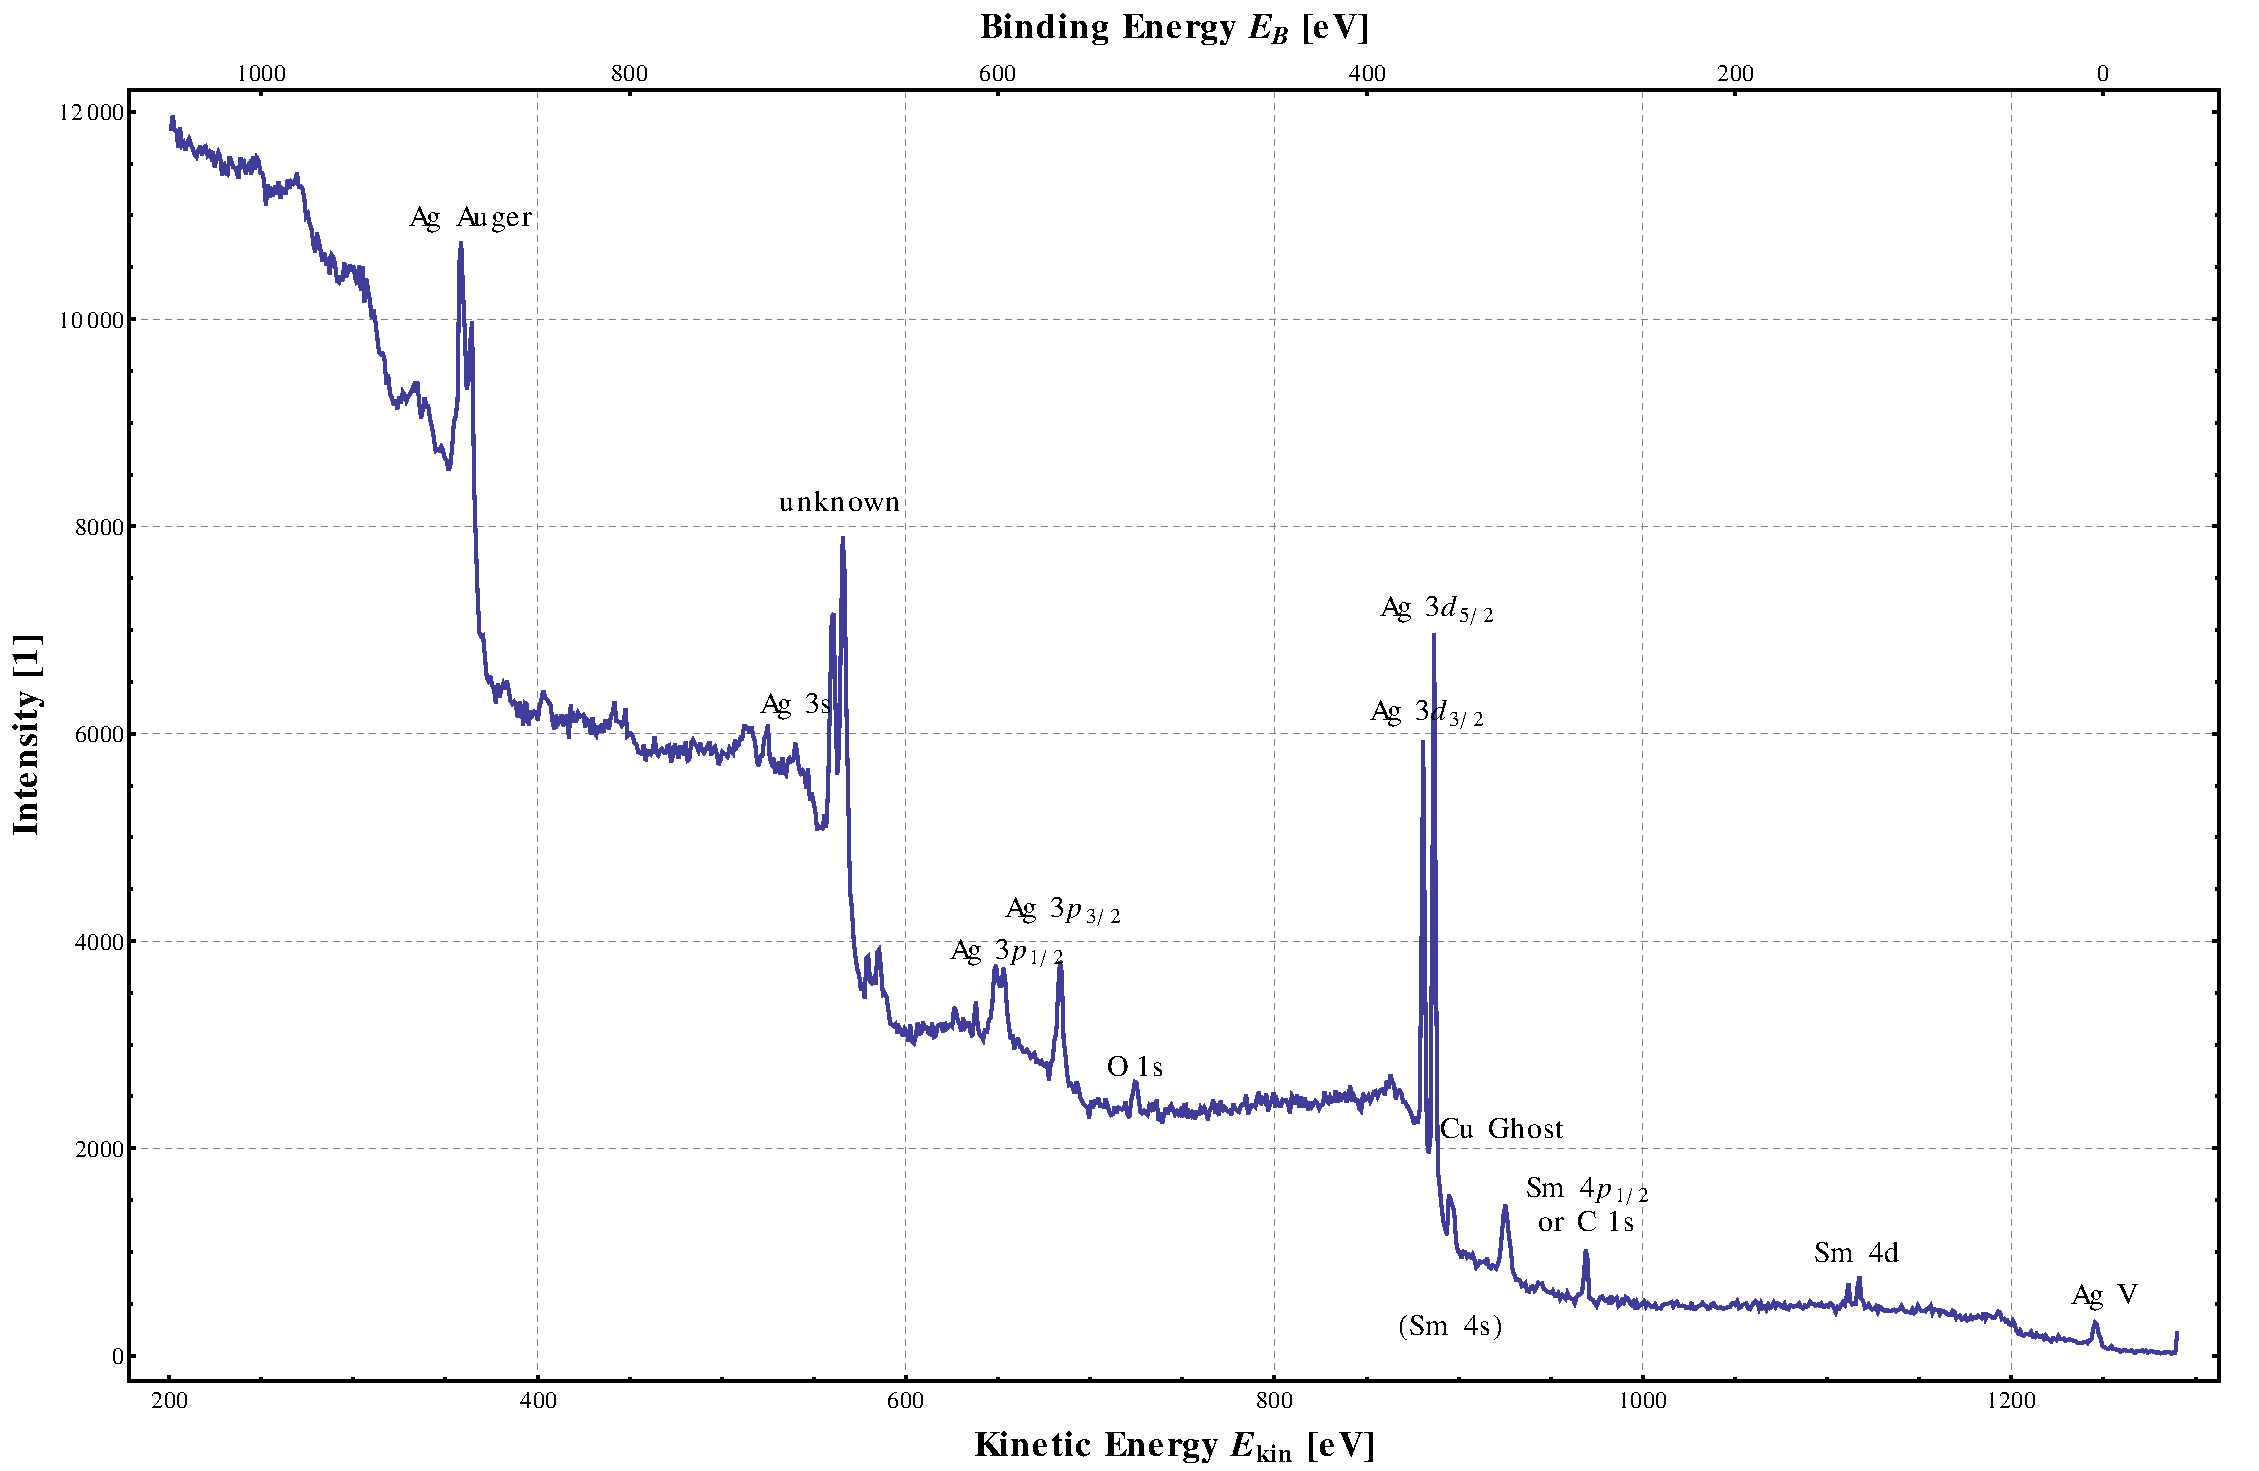
\includegraphics[scale=0.3]{img/silver_binding_mg}
\caption{Spectrum of silver sample taken with magnesium anode \label{fig:ag_mg}}
\end{figure}

\begin{table}[h]
\begin{center}
\begin{tabular}{lcccc}
\toprule
Measured $E_{B}$ [eV]        & Identification & Theoretical$E_{B}$ [eV] & Abs. Dev. [eV] & Dev. [\%]\\
\midrule
130.5 $\pm$ 1.5              & Sm $4d$        & 129                     & $1.5$          & $1.2$ \\
136.5 $\pm$ 1.5              & unknown        &                         &                &       \\
279.0 $\pm$ 1.5              & Sm $4p_{1/2}$  & 283                     & $-4.0$         & $-1.4$\\
279.0 $\pm$ 1.5              & C $1s$         & 285                     & $-6.0$         & $-2.1$\\
325.0 $\pm$ 1.9              & Cu Ghost       &                         &                &       \\
353.0 $\pm$ 1.5              & (Sm 4s)        & 349                     & $4.0$          & $1.1$ \\
361.5 $\pm$ 1.5              & Ag $3d_{5/2}$  & 368                     & $-6.5$         & $-1.8$\\
367.5 $\pm$ 1.5              & Ag $3d_{3/2}$  & 374                     & $-6.5$         & $-1.7$\\
523.5 $\pm$ 1.5              & O $1s$         & 525                     & $-1.5$         & $-0.3$\\
564.5 $\pm$ 1.9              & Ag $3p_{3/2}$  & 573                     & $-8.5$         & $-1.5$\\
595.0 $\pm$ 1.5              & Ag $3p_{1/2}$  & 604                     & $-9.0$         & $-1.5$\\
599.5 $\pm$ 1.5              & Ag $3p_{1/2}$  & 604                     & $-4.5$         & $-0.7$\\
682.5 $\pm$ 1.5              & unknown        &                         &                &       \\
688.0 $\pm$ 1.5              & unknown        &                         &                &       \\
708.0 $\pm$ 2.3              & Ag $3s$        & 719                     & $-11.0$        & $-1.5$\\
884.0 $\pm$ 1.9              & Ag Auger       & 896                     & $-12.0$        & $-1.3$\\
\bottomrule
\end{tabular}
\end{center}
\par
\caption{Binding energies obtained from silver spectrum taken with magnesium anode from figure~\ref{fig:ag_mg} \label{tab:ag_mg_ident}}
\end{table}

\subsection{Coin}

The coin sample is supposed to be a 10-DM memorial coin. According to~\cite{bank} these consist of $62.5\,\%$ and $37.5\,\%$. Since we were not able to identify the Fermi edge without reasonable doubt we used the Fermi edge of silver as a reasonable approximation, since it is supposed to consist mainly of silver.

Figure~\ref{fig:coin_al} shows an overview Al-K$_{\alpha}$ spectrum of the coin taken in the energy range of $200$--$1488.51\,$eV at a pass voltage of $50\,$V with 5 runs, a dwell time per point of $333\,$ms and 1300 points in the energy interval and figure~\ref{fig:coin_mg} shows an overview Mg-K$_{\alpha}$ spectrum of the coin in the energy range of $200$--$1290.02\,$eV and the same settings as for the scan with the aluminum anode.

As for all previous samples we compiled the photopeaks and, by comparison of the spectra, the Auger peaks. The data for the aluminum anode can be found in table~\ref{tab:coin_al_ident} and in table~\ref{tab:coin_mg_ident} for the magnesium anode.

In both spectra we again observe again the by now well-known shift between one and two percent of the binding energy to lower binding energies. Since shift is of about the same order of magnitude as for the silver sample, we see that using its Fermi edge as a reference was justified. 

In the spectra, we can identify silver and copper and as for the previous silver and samarium sample oxygen and samarium. The copper $3s$ and samarium $4d$ peak are located at the same position, so the peak is quite strong. In the range of very low binding energies  we can identify a very shallow and broad copper $3p_{1/2}$ peak.

The Mg-K$_{\alpha}$ spectrum again two points we were unable to identify, named X1 and X2, and one we tentatively identified as silver $3p_{1/2}$. Comparing the positions of the unknown peaks to those in table~\ref{tab:sm_mg_ident}, we see, that these peaks coincide. This implies, that we cannot identify the tentatively identified peak as silver $3p_{1/2}$, since we had to identify the peak X1 in table~\ref{tab;sm_mg_ident} as silver $3p_{1/2}$, too. This obviously makes no sense, since while it is reasonable that we find samarium on all samples, there is no obvious mechanism that could deposit silver on the samarium sample, more so on a freshly evaporated film.

The realization of coinciding peaks led us o the realization, that the samarium spectra and the spectra of the coin look almost the same. We thus rescaled both spectra, so that they are approximately the same height and plotted the spectra together in figure~\ref{sm-coin}. We see that, while they are not perfectly identical, which makes sense, since we can still detect some copper in the coins, the agreement is remarkable. This hints, that large quantities of samarium have found their way on the coin.


\begin{figure}[h]
\centering
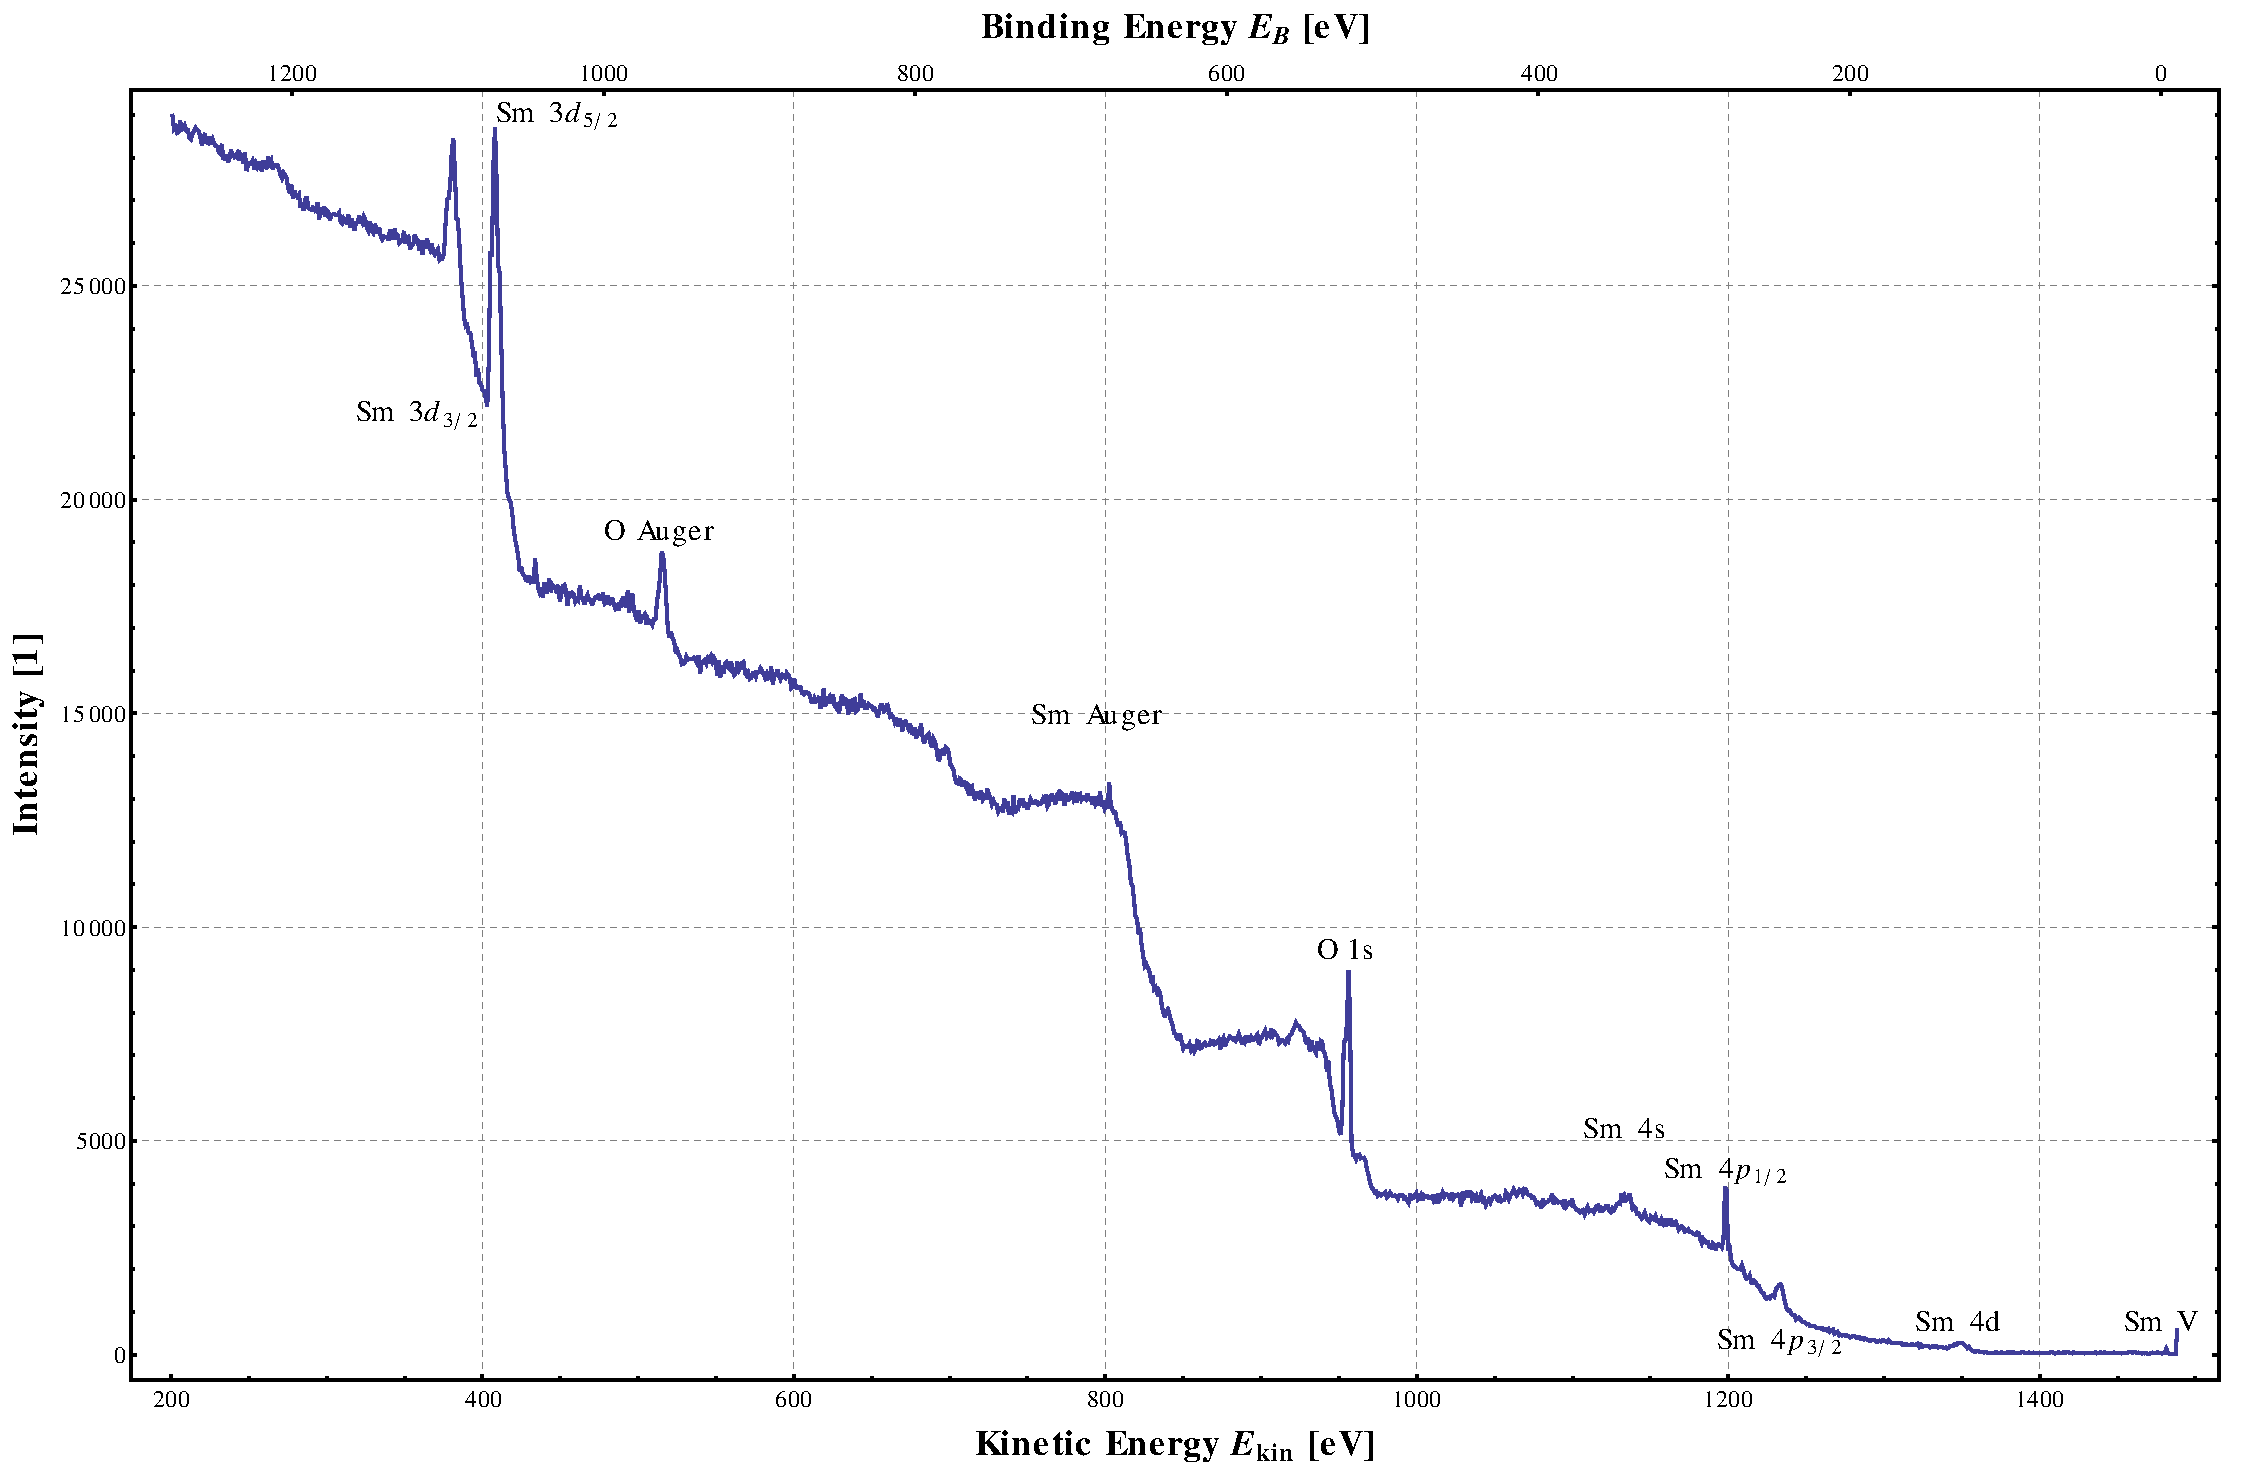
\includegraphics[scale=0.3]{img/samarium_binding_al}
\caption{Spectrum of the coin taken with aluminum anode \label{fig:coin_al}}
\end{figure}

\begin{figure}[h]
\centering
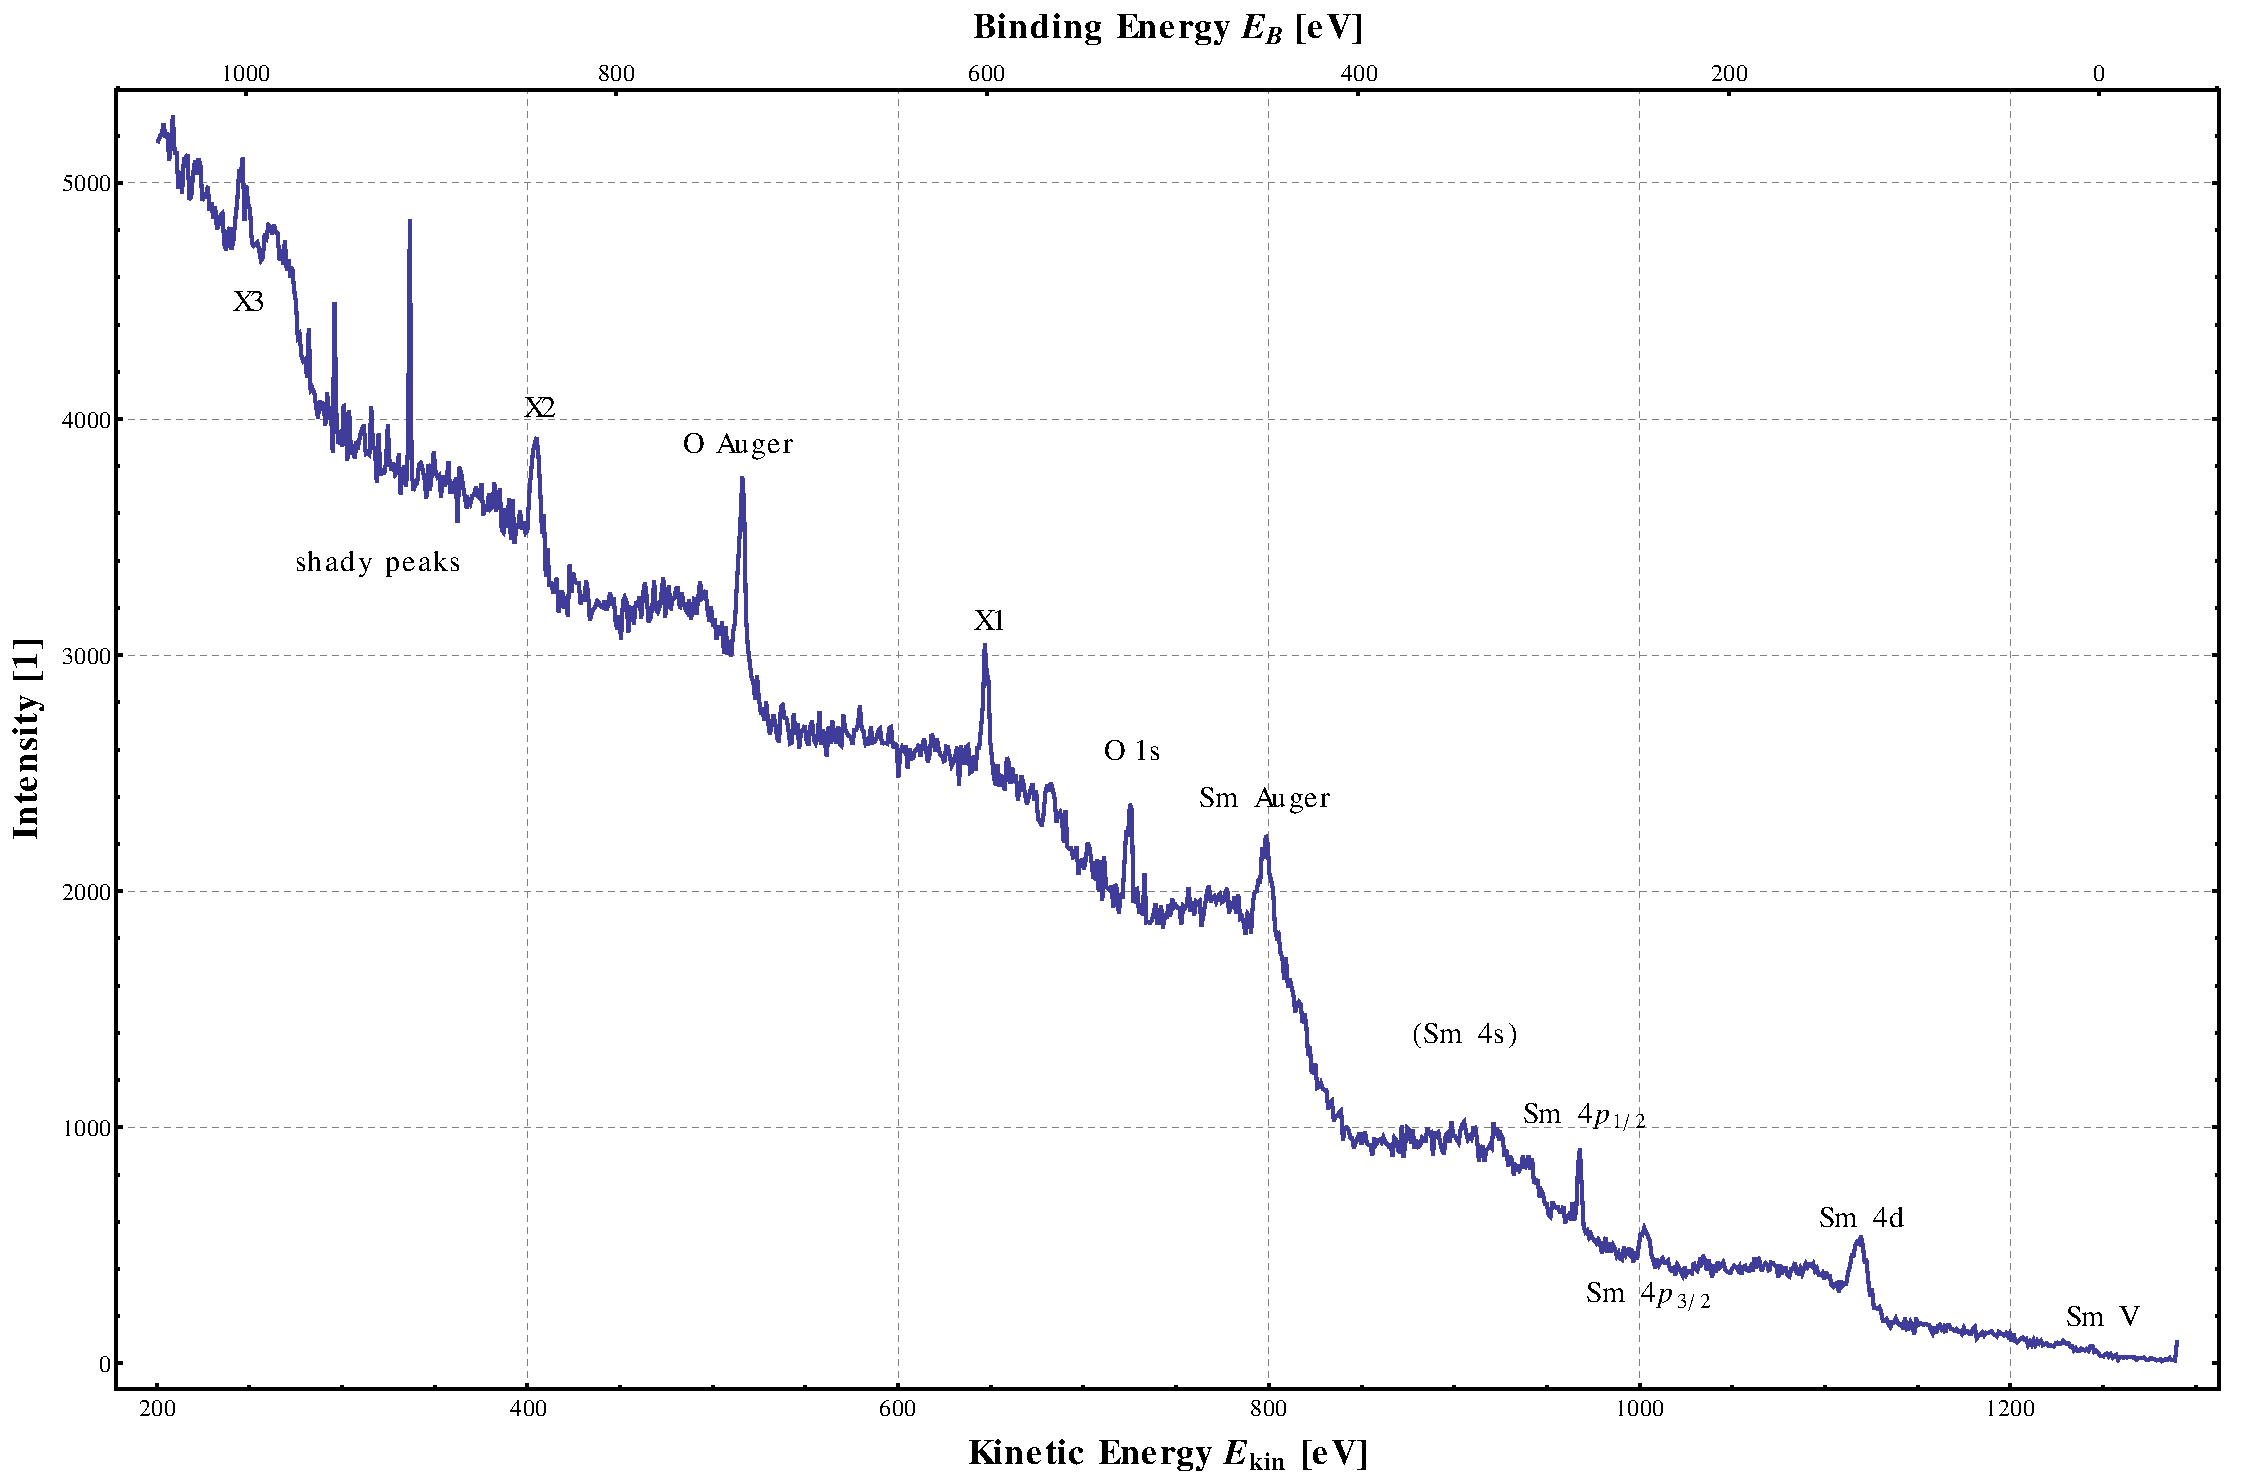
\includegraphics[scale=0.3]{img/samarium_binding_mg}
\caption{Spectrum of the coin taken with magnesium anode \label{fig:coin_mg}}
\end{figure}

\begin{table}[h]
\begin{center}
\begin{tabular}{lcccc}
\toprule
Measured $E_{B}$ [eV]      & Identification & Theoretical$E_{B}$ [eV] & Abs. Dev. [eV] & Dev. [\%]\\
\midrule
\phantom{00}72.0 $\pm$ 2.3 & Cu $3p_{1/2}$  & 77                      & $-5.0$         & $-6.5$   \\
\phantom{0}129.0 $\pm$ 2.3 & Cu $3s$        & 123                     & $6.0$          & $4.9$    \\
\phantom{0}129.0 $\pm$ 2.3 & Sm $4d$        & 129                     & $0.0$          & $0.0$    \\
\phantom{0}245.0 $\pm$ 1.9 & Sm $4p_{3/2}$  & 250                     & $-5.0$         & $-2.0$   \\
\phantom{0}278.0 $\pm$ 1.5 & Sm $4p_{1/2}$  & 283                     & $-5.0$         & $-1.8$   \\
\phantom{0}278.0 $\pm$ 1.5 & C $1s$         & 285                     & $-7.0$         & $-2.5$   \\
\phantom{0}360.5 $\pm$ 1.5 & Ag $3d_{5/2}$  & 368                     & $-7.5$         & $-2.0$   \\
\phantom{0}366.5 $\pm$ 1.9 & Ag $3d_{3/2}$  & 374                     & $-7.5$         & $-2.0$   \\
\phantom{0}522.5 $\pm$ 1.9 & O $1s$         & 531                     & $-8.5$         & $-1.6$   \\
\phantom{0}562.5 $\pm$ 2.3 & Ag $3p_{3/2}$  & 573                     & $-10.5$        & $-1.8$   \\
\phantom{0}594.0 $\pm$ 2.3 & Ag $3p_{1/2}$  & 604                     & $-10.0$        & $-1.7$   \\
\phantom{0}674.5 $\pm$ 1.5 & Sm Auger       & 682                     & $-7.5$         & $-1.1$   \\
\phantom{0}710.0 $\pm$ 2.3 & Ag $3s$        & 719                     & $-9.0$         & $-1.3$   \\
\phantom{0}920.0 $\pm$ 1.5 & Cu $2p_{3/2}$  & 933                     & $-13.0$        & $-1.4$   \\
\phantom{0}939.5 $\pm$ 1.5 & Cu $2p_{1/2}$  & 953                     & $-13.5$        & $-1.4$   \\
\phantom{0}963.0 $\pm$ 2.3 & O Auger        & 965                     & $-2.0$         & $-0.2$   \\
1069.0 $\pm$ 2.3           & Sm $3d_{5/2}$  & 1081                    & $-12.0$        & $-1.1$   \\
1096.0 $\pm$ 2.3           & Sm $3d_{3/2}$  & 1108                    & $-12.0$        & $-1.1$   \\
1120.0 $\pm$ 5.1           & Ag Auger       & 1129                    & $-9.0$         & $-0.8$   \\
\bottomrule
\end{tabular}
\end{center}
\par
\caption{Binding energies obtained from the coin taken with aluminum anode from figure~\ref{fig:coin_al} \label{tab:coin_al_ident}}
\end{table}

\begin{table}[h]
\begin{center}
\begin{tabular}{lcccc}
\toprule
Measured $E_{B}$ [eV]      & Identification  & Theoretical$E_{B}$ [eV] & Abs. Dev. [eV] & Dev. [\%]\\
\midrule
\phantom{00}74.0 $\pm$ 2.3 & Cu $3p_{1/2}$   & 77                      & $-3.0$         & $-3.9$\\
\phantom{0}130.0 $\pm$ 4.2 & Cu $3s$         & 123                     & $7.0$          & $5.7$ \\
\phantom{0}130.0 $\pm$ 4.2 & Sm $4d$         & 129                     & $1.0$          & $0.8$ \\
\phantom{0}279.0 $\pm$ 1.5 & Sm $4p_{1/2}$   & 283                     & $-4.0$         & $-1.4$\\
\phantom{0}279.0 $\pm$ 1.5 & C $1s$          & 285                     & $-6.0$         & $-2.1$\\
\phantom{0}450.0 $\pm$ 5.1 & Sm Auger        & 449                     & $1.0$          & $0.2$ \\
\phantom{0}523.5 $\pm$ 1.9 & O $1s$          & 531                     & $-7.5$         & $-1.4$\\
\phantom{0}600.0 $\pm$ 2.3 & (Ag $3p_{1/2}$) & 604                     & $-4.0$         & $-0.7$\\
\phantom{0}733.0 $\pm$ 2.3 & O Auger         & 745                     & $-12.0$        & $-1.6$\\
\phantom{0}844.0 $\pm$ 2.3 & X1              &                         &                &       \\
1000.0 $\pm$ 1.5           & X2              &                         &                &       \\
\bottomrule
\end{tabular}
\end{center}
\par
\caption{Binding energies obtained from the coin spectrum taken with magnesium anode fro figure~\ref{fig:coin_mg} \label{tab:coin_mg_ident}}
\end{table}

\begin{figure}[h]
\centering
\subfigure[ ]{
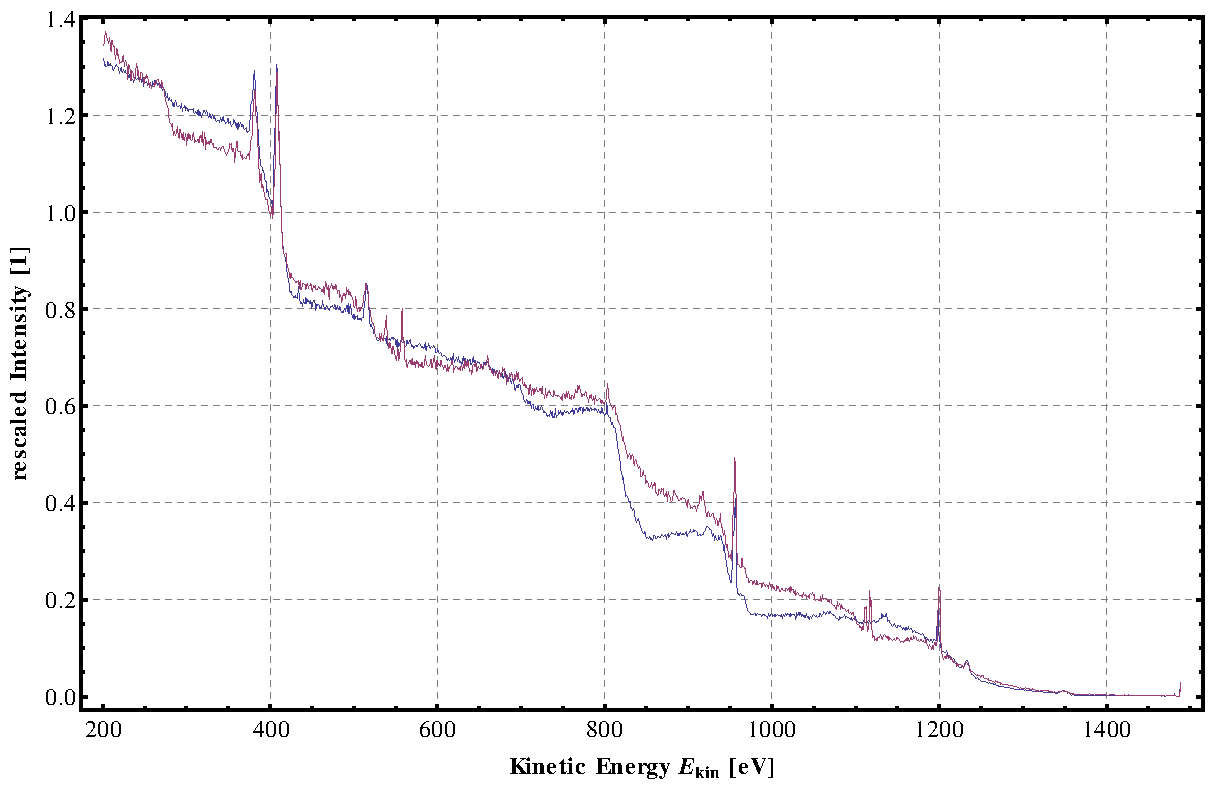
\includegraphics[scale=0.305]{img/samarium-coin_al}
\label{fig:smc_al}
}
\subfigure[ ]{
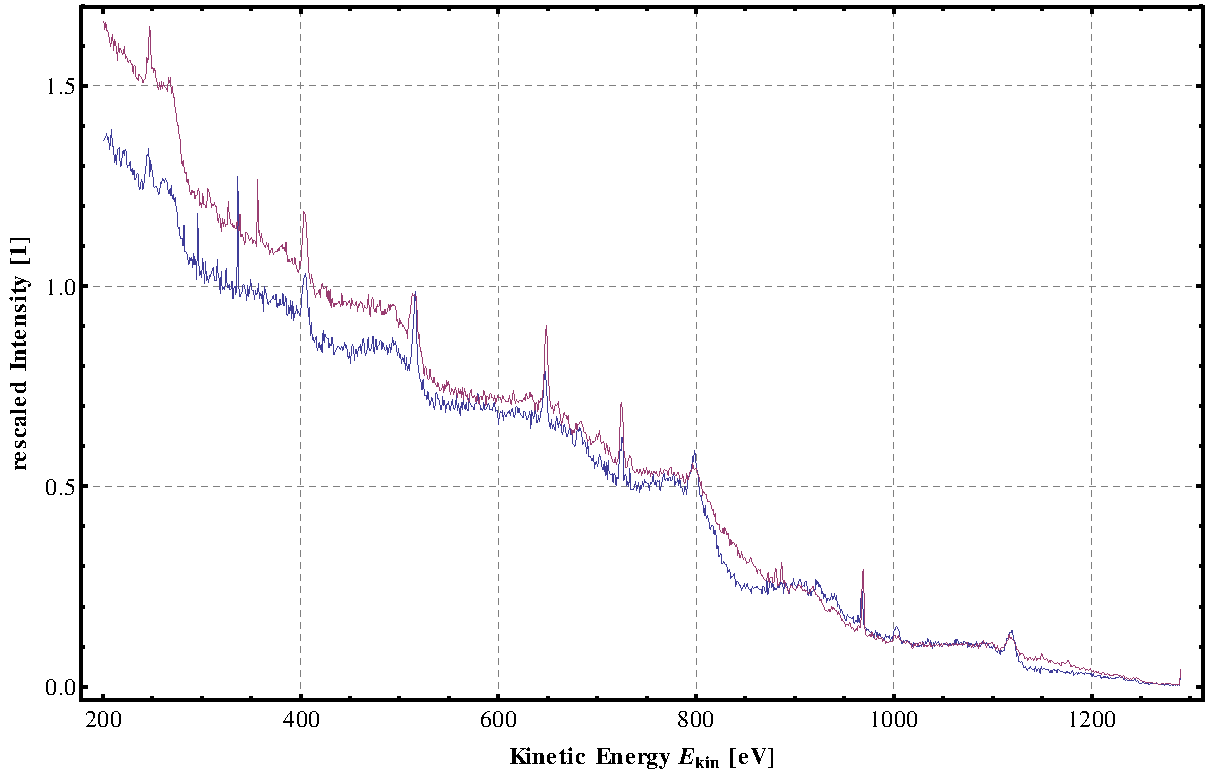
\includegraphics[scale=0.305]{img/samarium-coin_mg}
\label{fig:smc_mg}
}
\caption{Spectra for samarium and the coin, taken with aluminum anode \subref{fig:smc_al} and the magnesium anode \subref{fig:smc_mg}, rescaled to have approximately the same height. \label{fig:sm-coin}}
\end{figure}

\section{Conclusion}

We performed X-ray photoemission spectroscopy on several samples and successfully identified their photo- and Auger peaks and thus their composition. We observed that it is very surface sensitive and can be used to identify not only the composition of a material but also trace contaminants as oxygen or carbon.

The presence of strong oxygen peaks on all samples hints, that the experimental setup could be improved by adding other pumping systems, like ion getter or sublimation pumps. This would also be warranted if one would add methods of sample cleaning to the experiment, which we strongly recommend. The spectrum of the coin as far too strong similarities to the samarium spectrum and the silver spectrum, too, is contaminated with samarium, a sputter gun would thus greatly improve the experimental setup.

In the case of the addition of a sputter gun, the chamber would need to be opened, which would be a great chance to check the X-ray gun. Since the spectra get very high for electrons with low kinetic energies, far higher than expected from comparison with~\cite{handbook}, and the recommendation of the tutor to only use $200\,$eV as lower bound for energies, one might suspect low energy electrons leaking from the gun into the chamber, maybe through a crack in the gun's aluminum window.

Furthermore the experiment could be improved by adding a calibration task to the experiment, since we conclusively measured all binding energies lower than expected. A constant offset could easily be explained by a negatively charged sample. Also chemical shifts could have, and surely have an influence in our case, but we think that the relative shift by one or two percent is mostly a measurement artifact, due to the analyzer, which we cannot confirm, since the analyzer is mostly a black box to students.

\nocite{skript}
\nocite{handbook}
\nocite{booklet}
\nocite{nist}
\nocite{book}
\nocite{bank}

\bibliographystyle{plainnat}
\bibliography{xps}

\end{document}
